\section{Encryption Algorithms \& Security Definitions}
\label{sec:enc}
\noindent
In the previous section the notion of encryption was introduced (asymmetric and symmetric).
Here adversaries (i.e., attackers, or hackers) will be defined along with the specifications an algorithm must meet.

\begin{Def}[Adversaries]

    \label{def:adversaries}
    Adversaries are entities that attempt to break the security of a system.
    There are two types of adversaries:
    \begin{itemize}
        \item \textbf{Eavesdroppers:} Can only intercept and read messages.
        \item \textbf{Man-in-the-Middle (MitM):} Can intercept, read, and modify messages.
    \end{itemize}
\end{Def}

\begin{figure}[h!]
    \centering
    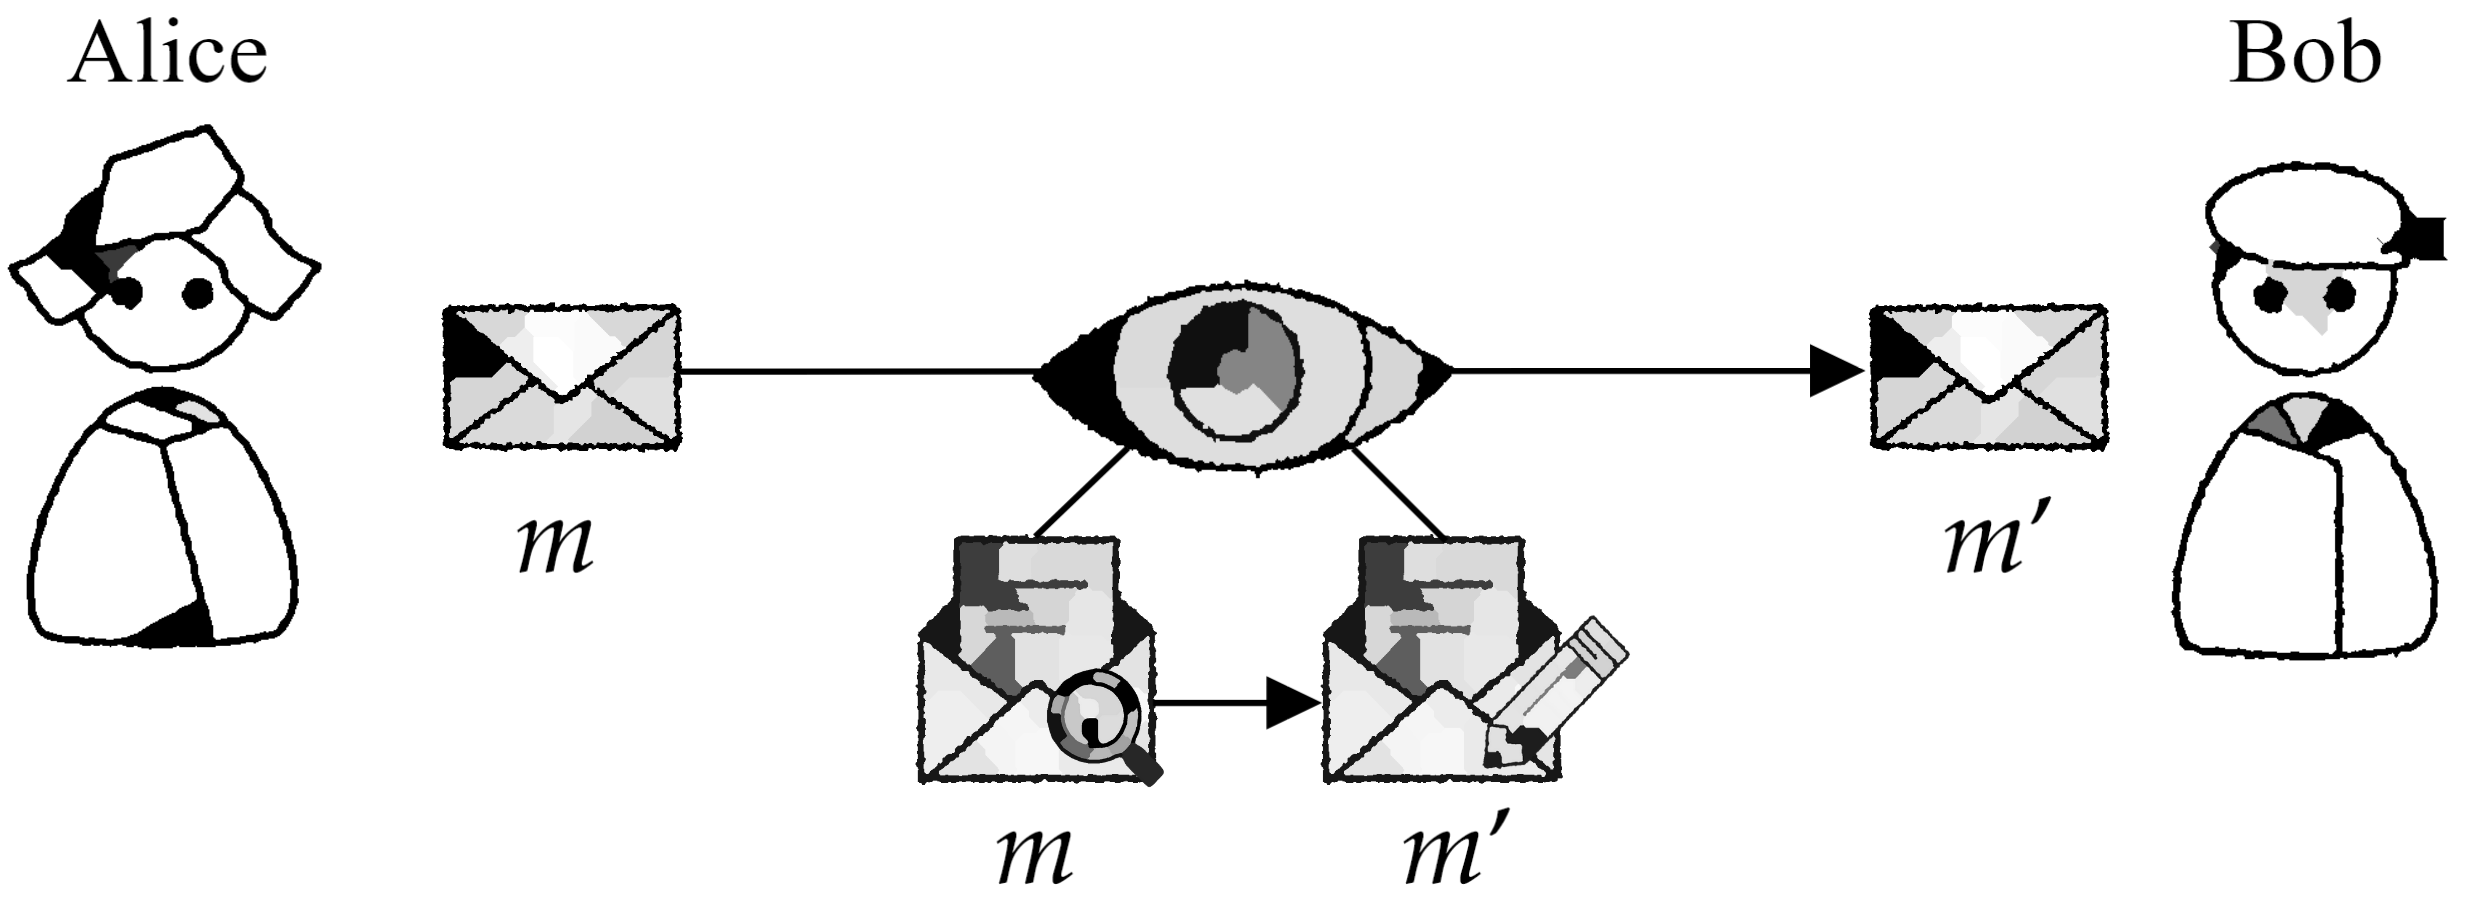
\includegraphics[width=.8\textwidth]{Sections/sec/enc/mitm.png}
    \caption{A MitM Attack, reading and altering the contents of $m$ and sending $m'$.}
    \label{fig:adv}
\end{figure}

\noindent
Instead plain variables $A$ and $B$, often Alice and Bob are used. There are other common for entities, learn more here:
\href{https://en.wikipedia.org/wiki/Alice_and_Bob}{https://en.wikipedia.org/wiki/Alice\_and\_Bob}.

\newpage 
\begin{Def}[Security Definitions]

    \label{def:security_definitions}
    Security definitions formalize the properties a system must satisfy to resist adversarial attacks. These include:
    \begin{itemize}
        \item \textbf{Confidentiality:} Ensures that adversaries cannot learn the contents of the message.
        \item \textbf{Integrity:} Guarantees that adversaries cannot alter the message without detection.
        \item \textbf{Authenticity:} Verifies that the message originates from the claimed sender and has not been tampered with.
    \end{itemize}
\end{Def}

\begin{theo}[Kerckhoffs's Principle]

    \label{theo:kerckhoffs}
    \begin{center}
        \Large\textit{``Il faut qu'il n'exige pas le secret, et qu'il puisse sans inconvénient tomber entre
        les mains de l'ennemi.''}
    \end{center}

    \vspace{1em}
    \normalsize

    \noindent
    \textbf{Literal translation}: [The method] must not be required to be secret, and it
    must be able to fall into the enemy's hands without causing inconvenience \cite{joyofcryptography}.
\end{theo}

\begin{figure}[h!]
    \centering
    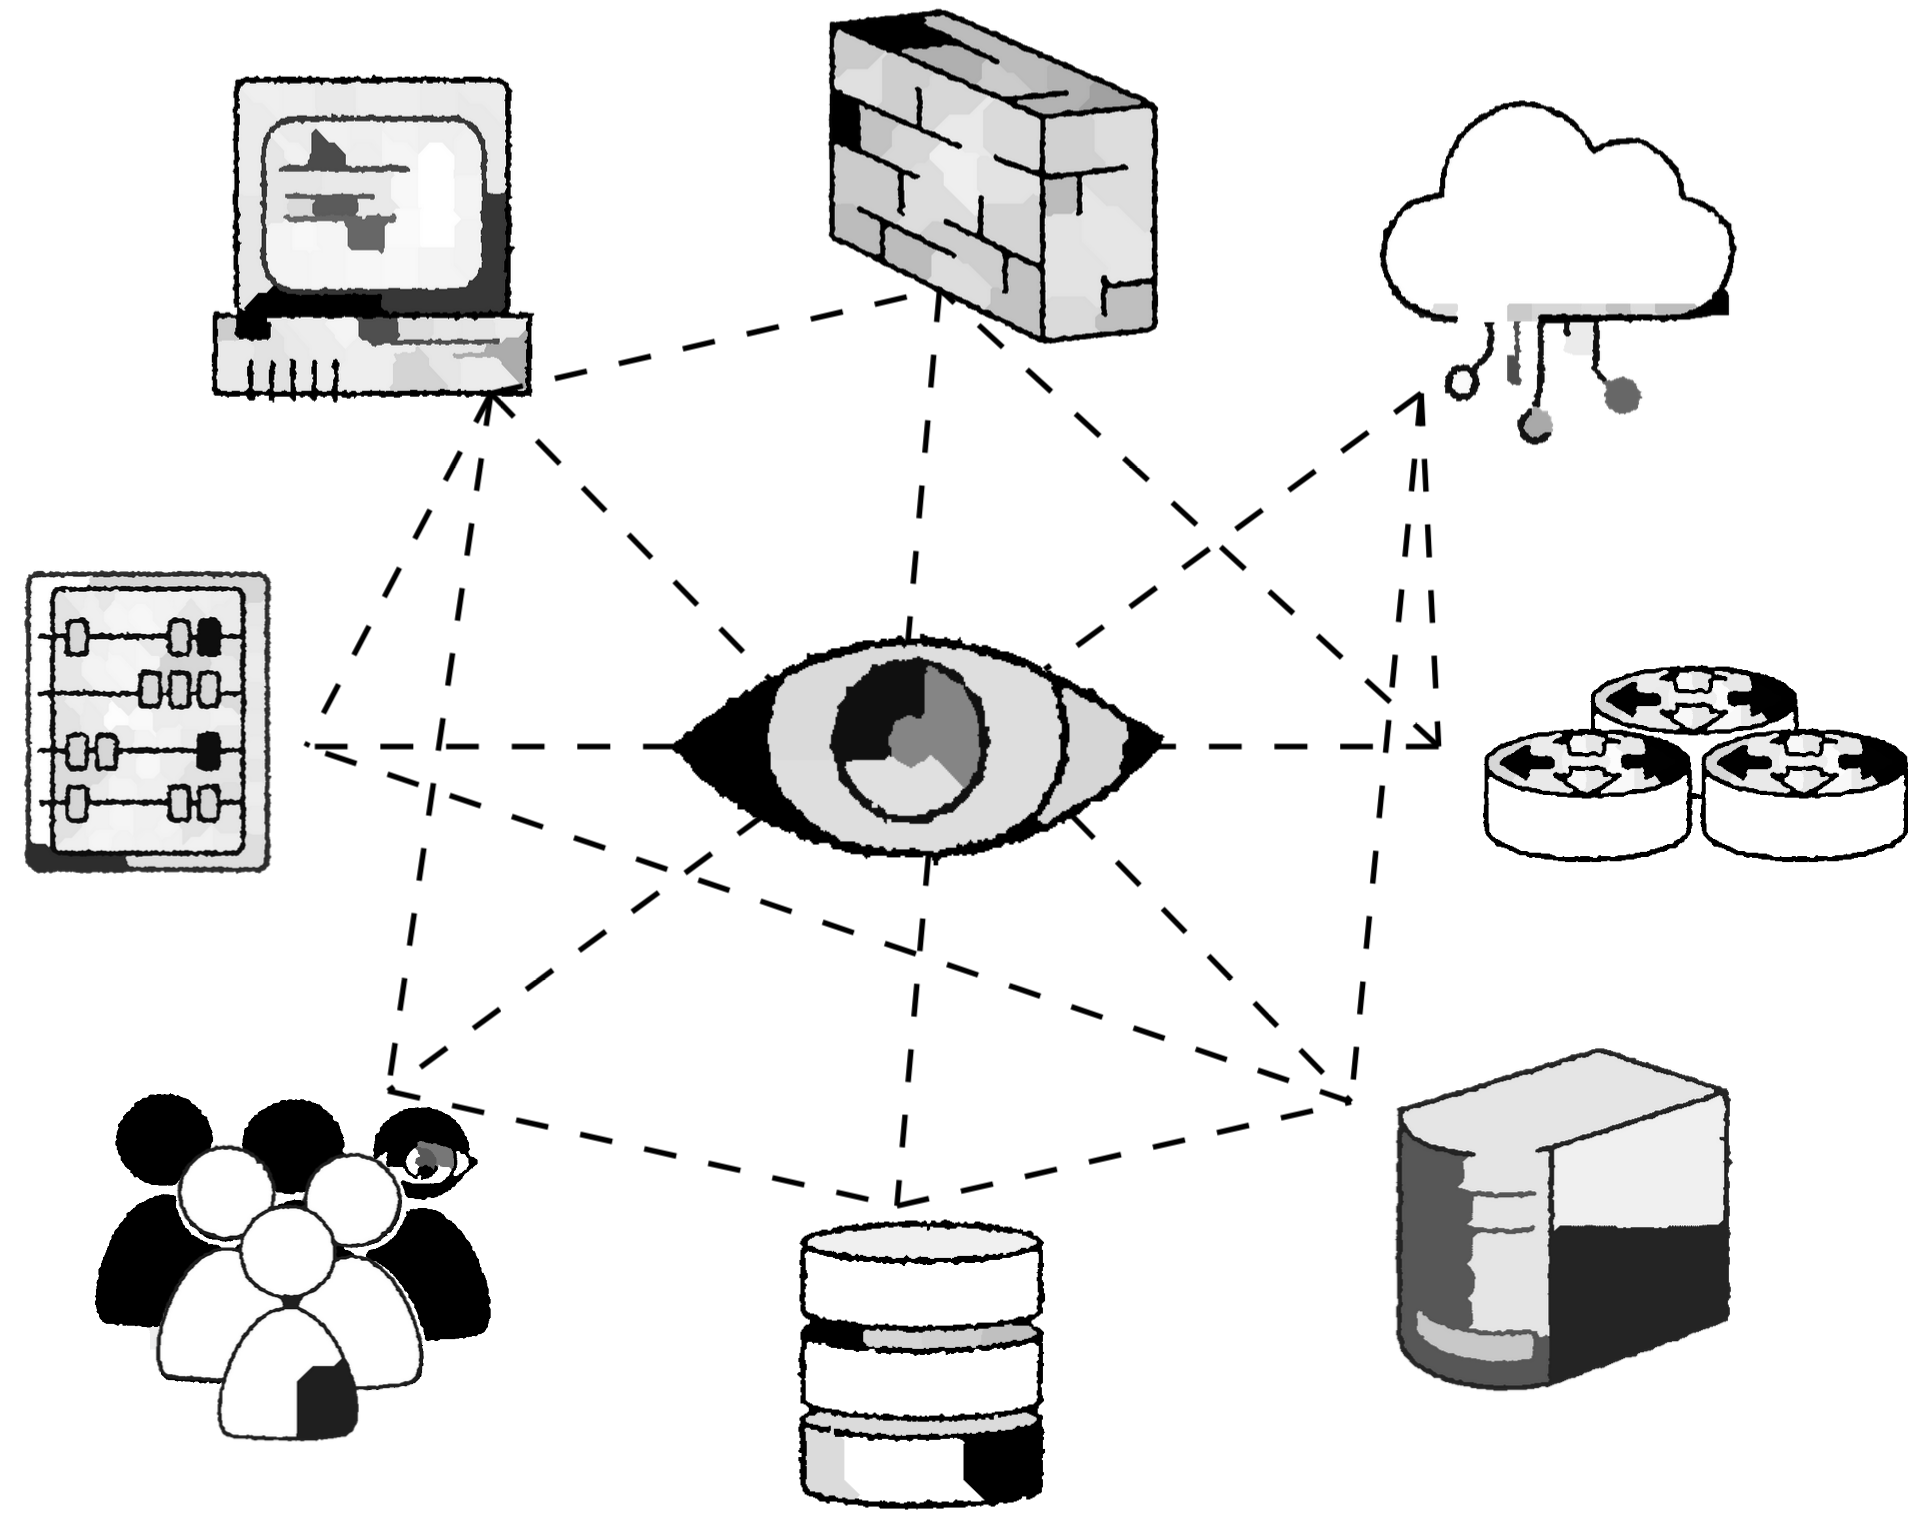
\includegraphics[width=.6\textwidth]{Sections/sec/enc/enemy.png}
    \caption{Kerckhoffs's Principle, an adversary's unbounded sight.}
    \label{fig:kerckhoffs}
\end{figure}

\noindent
I.e., \textbf{The adversary knows all}---the algorithm, the architecture, an insider, any exploit---all communication is naked, visible on the wire.
Though despite all, is secure. This is the essence of Kerckhoffs's Principle.

\newpage

\begin{Def}[Non-cryptographic Security]

    \label{def:non_crypto}
    A system which does not follow Kerkhoff's Principle: security through obscurity (hiding the algorithm) is not a cryptographic. As 
    if any rosetta stone is found, the system is compromised.
\end{Def}

\vspace{-1em}
\begin{Note}
    \textbf{Note}: The rosetta stone was a slab of stone found in 1799, which helped decipher Egyptian hieroglyphics. I.e., a key between languages.
    Learn more: \href{https://en.wikipedia.org/wiki/Rosetta_Stone}{https://wikipedia.org/rosetta\_stone}.
\end{Note}

\noindent
The rest of the section will cover methods used over centuries to attempt to secure messages.

\begin{theo}[Caesar Cipher]

    \label{theo:caesar_cipher}
    The Caesar Cipher is a non-cryptographic scheme, named after Julius Caesar, dating back 45BC to protect military communications.
    Each letter in the plaintext is shifted $x$ places down the alphabet. E.g., $x= 3$, `A'=`D', `B'=`E', and so on. \hfill \cite{timour2019crypto}
\end{theo}

\vspace{-1em}
\begin{Note}
    \textbf{Note}: Here is a fun online tool to try the Caesar Cipher: \href{https://cryptii.com/pipes/caesar-cipher}{https://cryptii.com/caesar-cipher}.
\end{Note}

\begin{theo}[Vigenère Cipher]

    \label{theo:vigenere_cipher}
    The Vigenère Cipher is a non-cryptographic scheme, created in mid-1500's by italian cytologist Giovan Battista Bellaso,
    later popularized and misattributed to Blaise de Vigenère. It addressed the Caesar Cipher's weakness by using attributing odd and even digit places to different Caesar Ciphers.

    This was aimed to stop frequency analysis attacks, as for instance, `E' is the most common letter in English. If a letter is repeated at high frequency, it is likely `E'. \hfill \cite{timour2019crypto}
\end{theo}
\begin{figure}[h!]
    \centering
    \[
    \begin{array}{c|c|c|c|c|c|c|c|c|c|c|c|c|c|c|c|c|c|c|c|c|c|c|c|c|c|c}
    
    0 & a & b & c & d & e & f & g & h & i & j & k & l & m & n & o & p & q & r & s & t & u & v & w & x & y & z \\ \hline\hline
    1 & f & g & h & i & j & k & l & m & n & o & p & q & r & s & t & u & v & w & x & y & z & a & b & c & d & e \\ \hline
    2 & k & l & m & n & o & p & q & r & s & t & u & v & w & x & y & z & a & b & c & d & e & f & g & h & i & j \\
    \end{array}
    \]
    \caption{Vigenère Cipher Table: row 0 is the key, 1 even, and 2 odd shift.}
    \label{fig:caesar_shift_table}
\end{figure}

\noindent
For example ``Coffee'' would be ``hykpjo'' deterring frequency analysis of the letter `E'.

\newpage 

\begin{Func}[Key \& String Length ($\lambda,\|a\|$)]

    \vspace{-.5em}
    \label{func:bit_length}
    The rest of the text may denote `$\lambda$' (lambda) as the bit length of the key. E.g., $\lambda = 8$ bits, which in in binary may hold $2^8 = 256$ values ($[0000\ 0000]_2\text{-}[1111\ 1111]_2$).
    The $\lambda$ is variable is often called the \textbf{security parameter}.\\
    \noindent
    \rule{\textwidth}{0.4pt}
    \textbf{For ease of notation}, $\|a\|$ denotes the length of a character or binary string $a$. E.g., $\|a\| = 5$ for the string $a = \text{``hello''}$
    (the use of which will always be explicit).
    \hfill \cite{joyofcryptography}
\end{Func}

\begin{Def}[One-Time Pad (OTP)]

    \label{def:one_time_pad}
    OTP, also known as the \textbf{Vernam Cipher} is a cryptographic scheme, invented by Gilbert Vernam in 1919.
    Earlier depictions though date back to 1882 by Frank Miller on telegraphy.\\
    \noindent
    \rule{\textwidth}{0.4pt}
    \textbf{Security Definition}: Confidentiality is guaranteed if the key is used only once.
\end{Def}

\begin{Func}[One Time Pad - \texttt{Enc(m, k)} \& \texttt{Dec(k, c)}]

    \vspace{-.5em}
    \label{func:otp}
    \noindent
    Let function $k\leftarrow\{0,1\}^{\lambda}$ generate keys $k$:
    \begin{itemize}
        \item $\{0,1\}$ denotes the set of possible inputs.
        \item $k$ is a random bit string of length $\lambda$ bits consisting of 0's and 1's. E.g., $\lambda = 8$ then $k = [1010\ 1101]_2$ is a possible output.
        \item $\{0,1\}^{\lambda}$ should be a uniform distribution, i.e., each bit is equally likely to be 0 or 1.
    \end{itemize}
    \noindent
    Let $m$ be and $c$ be an encrypted message, both length $\lambda$ bits. Then: 
    \begin{itemize}
        \item $c\leftarrow \text{Enc}(m,k) := m\oplus k$. (Encryption)
        \item $m\leftarrow \text{Dec}(k,c) := c\oplus k$. (Decryption)
    \end{itemize}

    \noindent
    Where $\oplus$ denotes the XOR operation $(1\oplus1=0; 0\oplus1=1; 1\oplus0=1; 0\oplus0=0)$.
\end{Func}

\[
c\gets\text{Enc}(m,k) :=
\begin{cases}
\begin{array}{r@{\;}r}
\textcolor{Wine}{0011\ 0100\ 1101\ 1000\ 1111} & \hspace{1em} (m) \\[2pt]
\oplus\ \textcolor{Wine}{1110\ 1010\ 0110\ 1000\ 1101} & \hspace{1em} (k) \\[2pt]
\hline
\textcolor{Wine}{1101\ 1110\ 1011\ 0000\ 0010} & \hspace{1em} (c)
\end{array}
\end{cases}
\text{(Encryption)}
\]
\[
m \gets \text{Dec}(c,k) :=
\begin{cases}
\begin{array}{r@{\;}r}
\textcolor{Wine}{1101\ 1110\ 1011\ 0000\ 0010} & \hspace{1em} (c) \\[2pt]
\oplus\ \textcolor{Wine}{1110\ 1010\ 0110\ 1000\ 1101} & \hspace{1em} (k) \\[2pt]
\hline
\textcolor{Wine}{0011\ 0100\ 1101\ 1000\ 1111} & \hspace{1em} (m)
\end{array}
\end{cases}
\text{(Decryption)}
\]
\newpage 

\noindent
The larger the key, the more secure the scheme becomes, as smaller keys have a higher probability of being brute-forced by generating
all possible keys.

\begin{theo}[Computational Security]

    \label{theo:computational_security}
    \textbf{Computational Security} is a security definition that guarantees that the adversary cannot break the scheme in a reasonable amount of time.
    In todays standards, exponential time algorithms are considered infeasible, (e.g., $O(2^{\lambda})$ time complexity).
\end{theo}

\vspace{-2em}
\begin{figure}[h!]
    \centering
    \[
    \begin{tabular}{ll}
        \textbf{Efficient algorithm known:} & \textbf{No known efficient algorithm:} \\
        Computing GCDs & Factoring integers \\
        Arithmetic mod \( N \) & Computing \( \phi(N) \) given \( N \) \\
        Inverses mod \( N \) & Discrete logarithm \\
        Exponentiation mod \( N \) & Square roots mod composite \( N \)
    \end{tabular}
    \]
    \caption{Comparison of problems with known efficient algorithms and those without \cite{joyofcryptography}.}
    \label{fig:efficient_vs_no_algorithm}
\end{figure}

\begin{Def}[Known \& Chosen Plaintext Attacks]

    \textbf{Known Plaintext Attack (KPA)}:\\
    The adversary has access to one or more known unencrypted and encrpyted message pairs.\\

    \vspace{-.5em}
    \noindent
    \textbf{Chosen Plaintext Attack (CPA)}:\\
    The adversary encrypts plaintext of their choosing to analyze the corresponding ciphertexts.
\end{Def}

\noindent
The Caesar Cipher and Vigenère Cipher are both vulnerable to plaintext attacks. The One-Time Pad (OTP), becomes vulnerable if the key is small or reused.


\begin{Def}[Block Ciphers]

    \label{theo:block_cipher}
    A cryptographic scheme that separates and encrypts fixed-length blocks of plaintext into ciphertext. Let $\beta$ (beta) be the block size, and $\lambda$ the key length.
    Then for a set of $B$ blocks and message $M$: $\sum_{b\in B} \beta = \|M\|$ (the sum of all blocks equals the length of the message).\\
    We define $\text{Enc}_\lambda(M,\beta)$, $\text{Dec}_\lambda(C,\beta)$, $C$ as the set of ciphertext blocks, s.t.:
    \begin{align*}
        \text{Enc}_\lambda(M,\beta) \rightarrow C : b\in B \mapsto c\in C\\
        \text{Dec}_\lambda(C,\beta) \rightarrow M : c\in C \mapsto b\in B\\
    \end{align*} 

    \vspace{-1em}
    \noindent
    Where $\lambda :=\{(b,c),\dots\}, \text{a dictionary of unique message block to ciphertext pairs (bijection)}$.
\end{Def}

\newpage 

\noindent
The below figure demonstrates use of a block cipher with a block size of 2, using the Electronic Codebook Mode (ECB).
\begin{figure}[h!]
    \centering
    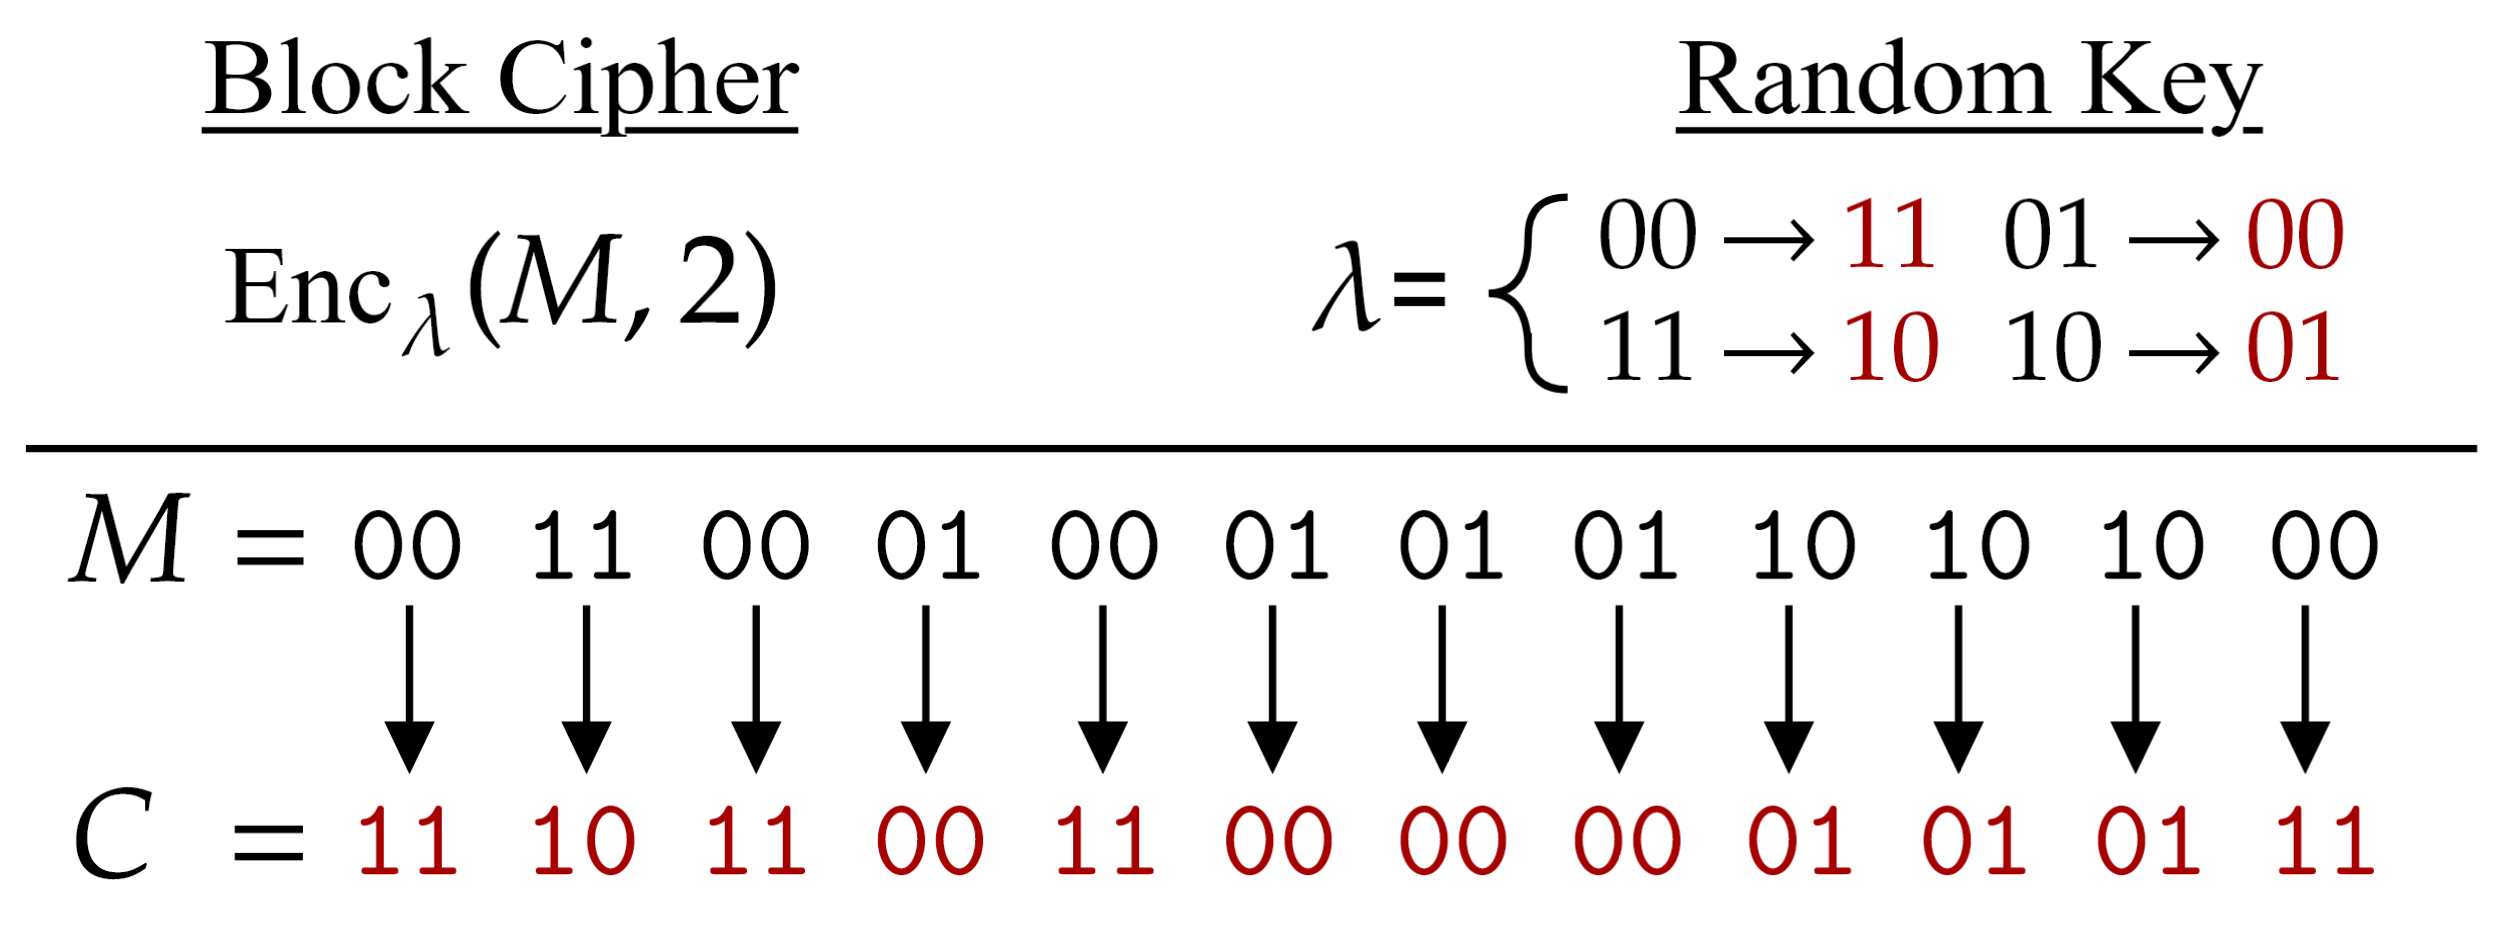
\includegraphics[width=.8\textwidth]{Sections/sec/enc/block.png}
    \caption{Electronic Codebook Mode (ECB) with a block size of 2 \cite{essex2024encrypting}.}
    \label{fig:block_cipher}
\end{figure}

\noindent
Though in its simplicity falls to the same weakness as the Caesar Cipher, as identical plaintext blocks will encrypt to the same ciphertext block.

\begin{figure}[h!]
    \centering
    \rule{\textwidth}{0.4pt}

    \vspace{1em}
    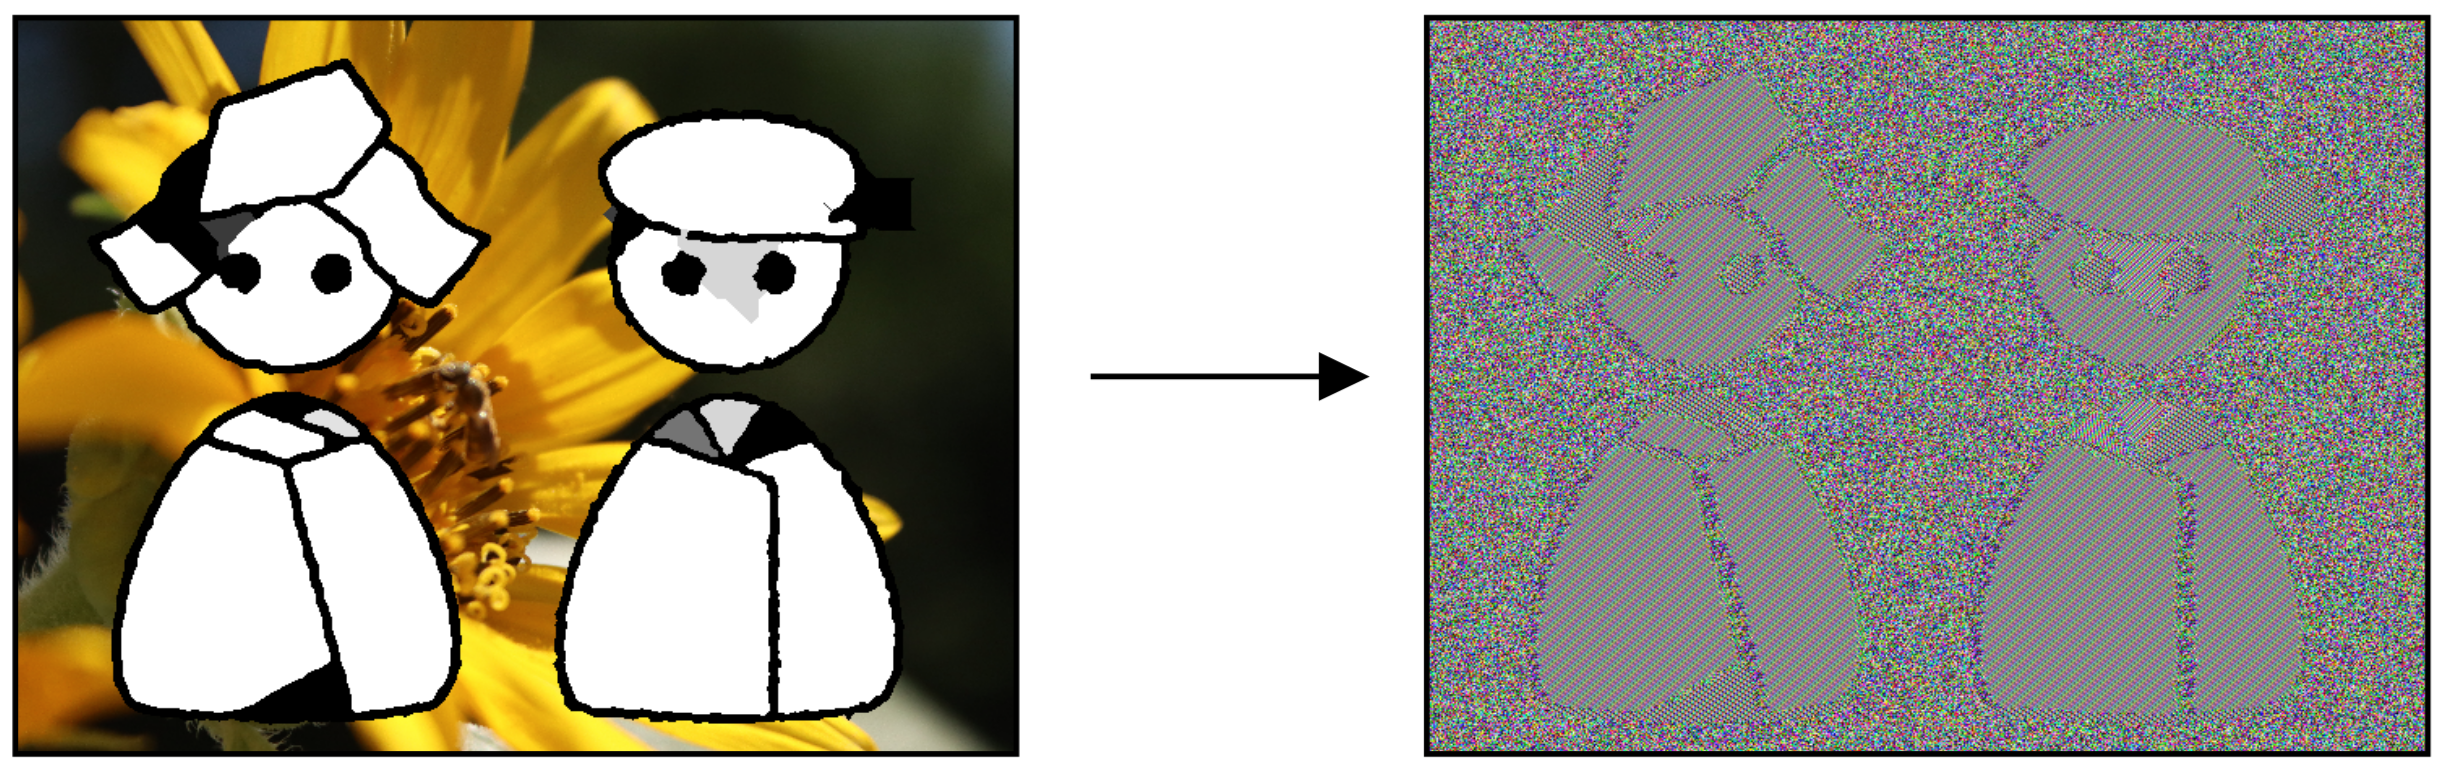
\includegraphics[width=.8\textwidth]{Sections/sec/enc/ecb.png}
    \rule{\textwidth}{0.4pt}
    \caption{An unencrypted image (left) and the same image encrypted with ECB (right).}
    \label{fig:block_cipher}
\end{figure}

\noindent
Here the image on the right is still partially recognizable, as when ECB encountered white space, it encrypted it to the same block.
Shockingly the popular video conferencing software Zoom used ECB during the 2020 COVID-19 pandemic, of which now has been patched.

\vspace{1em}
\begin{Def}[Cipher Block Chaining (CBC)]

    \label{theo:cipher_block_chaining}
    CBC encrypts blocks of plaintext into ciphertext. CBC uses a \textbf{Initialization Vector (IV)} to start the chain of XORing.
    The IV is XORed with the first plaintext block. Each XOR is indexed into the key value pair dictionary $\lambda$. The result is the cypher text block.
    Then the ciphertext block XORs with the next plaintext block and so on. \hfill \cite{nist80038a}\\
    \noindent
    \rule{\textwidth}{0.4pt}
    \textbf{Security Definition}: Confidentiality. Integrity and Authenticity are not guaranteed.
\end{Def}

\newpage 

\noindent
The below figure demonstrates use of a block cipher with the Cipher Block Chaining Mode (CBC).

\begin{figure}[h!]
    \centering
    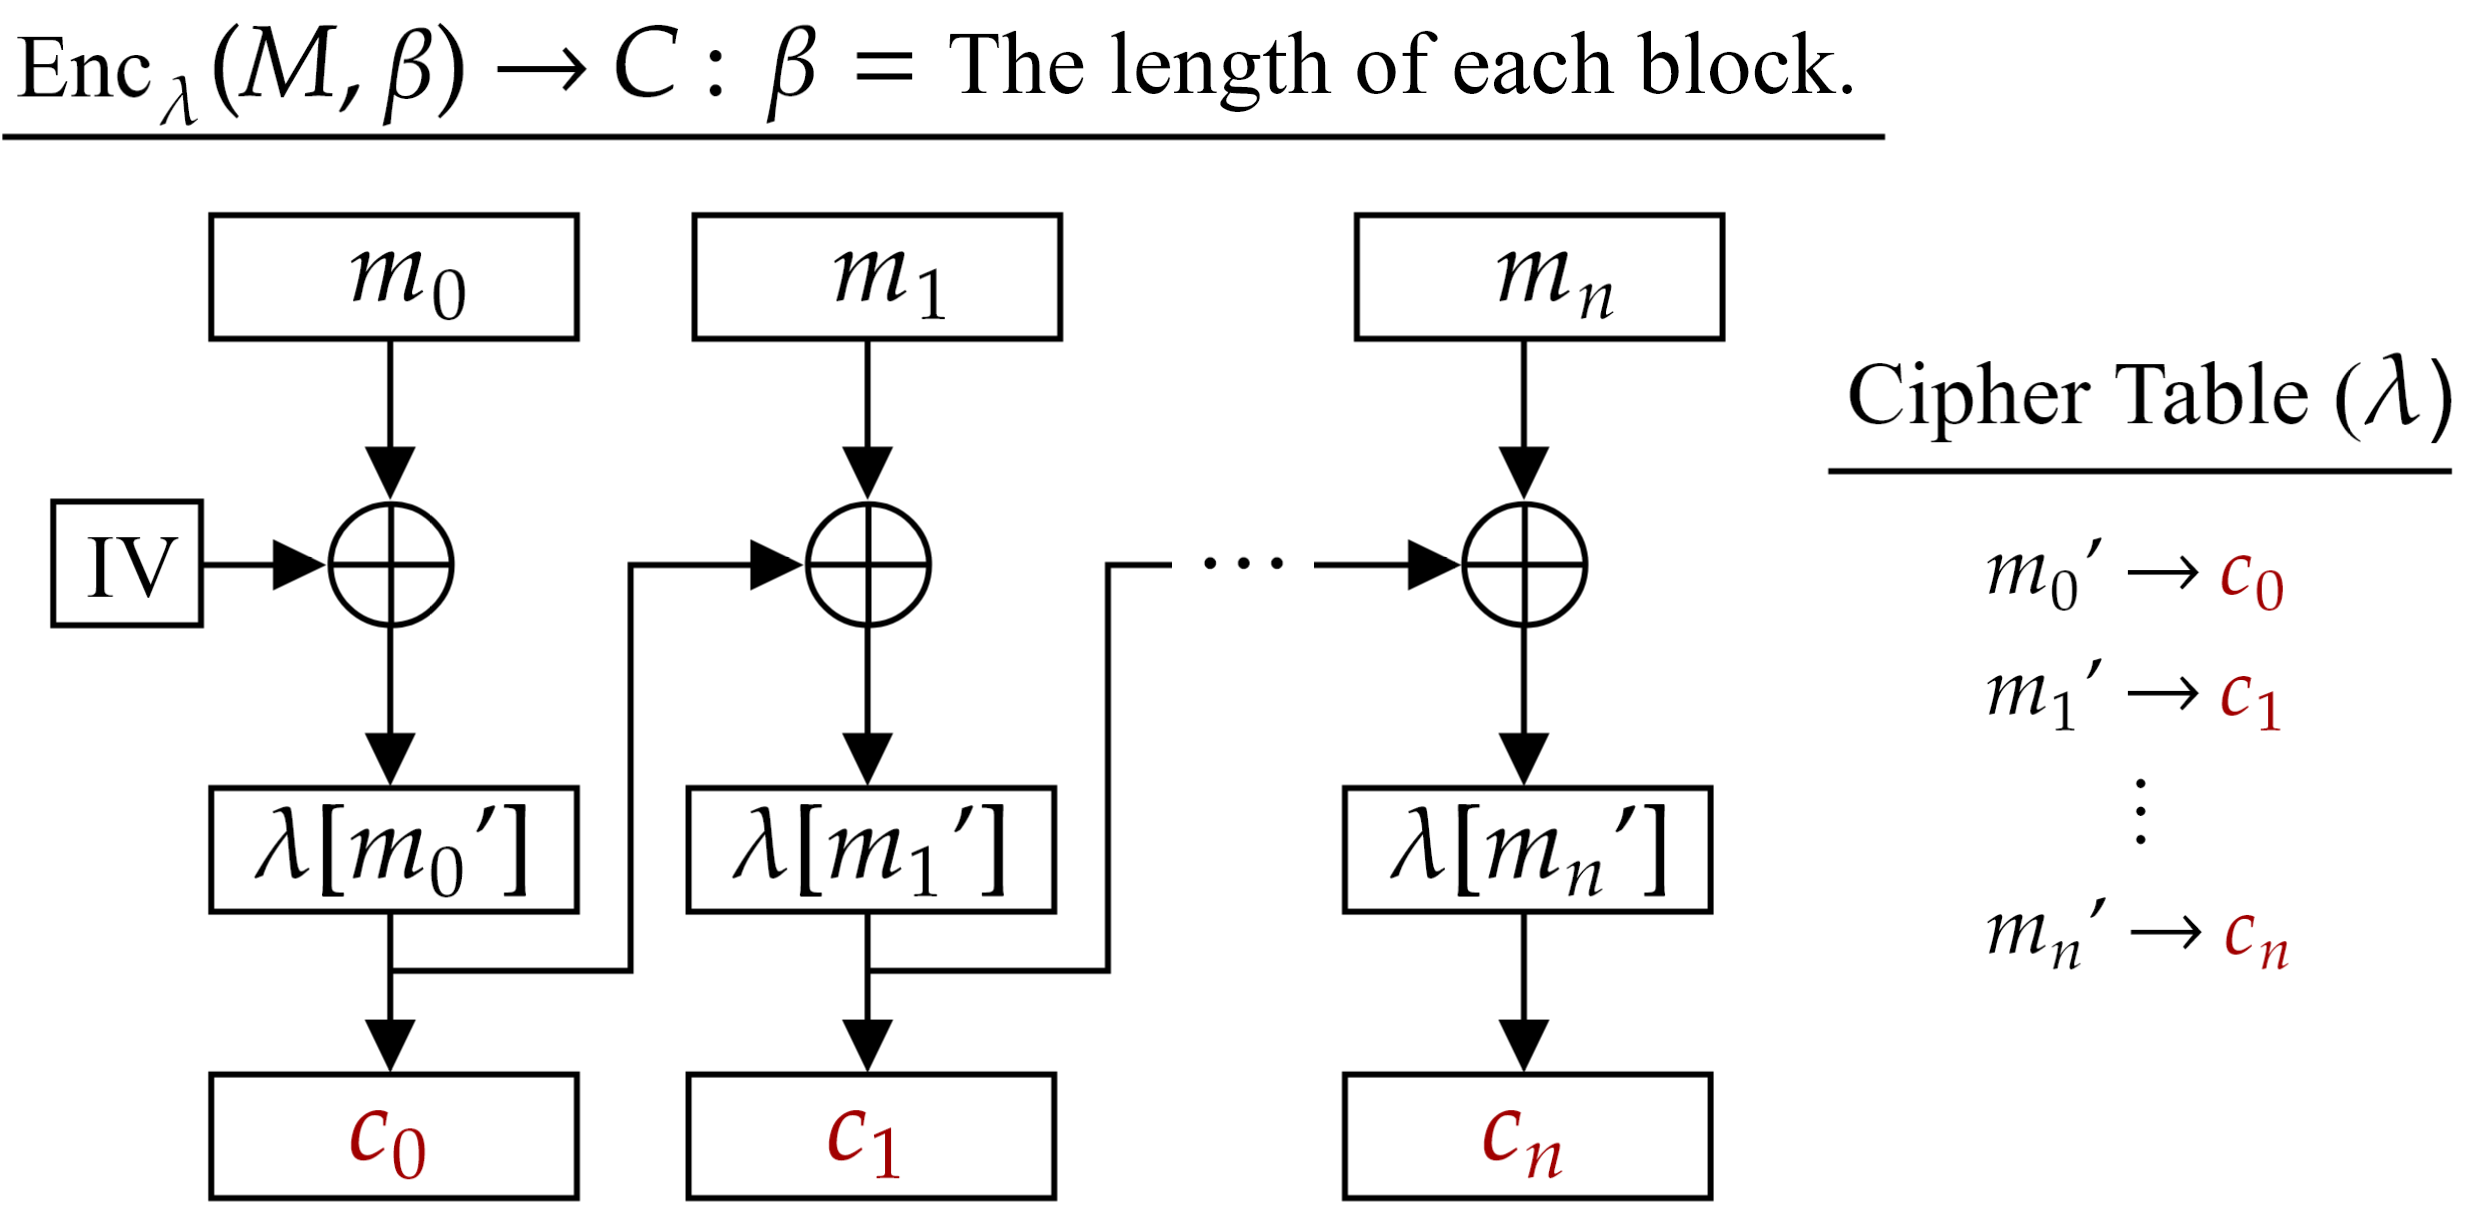
\includegraphics[width=.8\textwidth]{Sections/sec/enc/cbc.png}
    \caption{A block cipher utilizing the Cipher Block Chaining Mode (CBC) method. \cite{essex2024encrypting}.}
    \label{fig:block_cipher}
\end{figure}

\vspace{-1em}
\begin{figure}[h!]
    \centering
    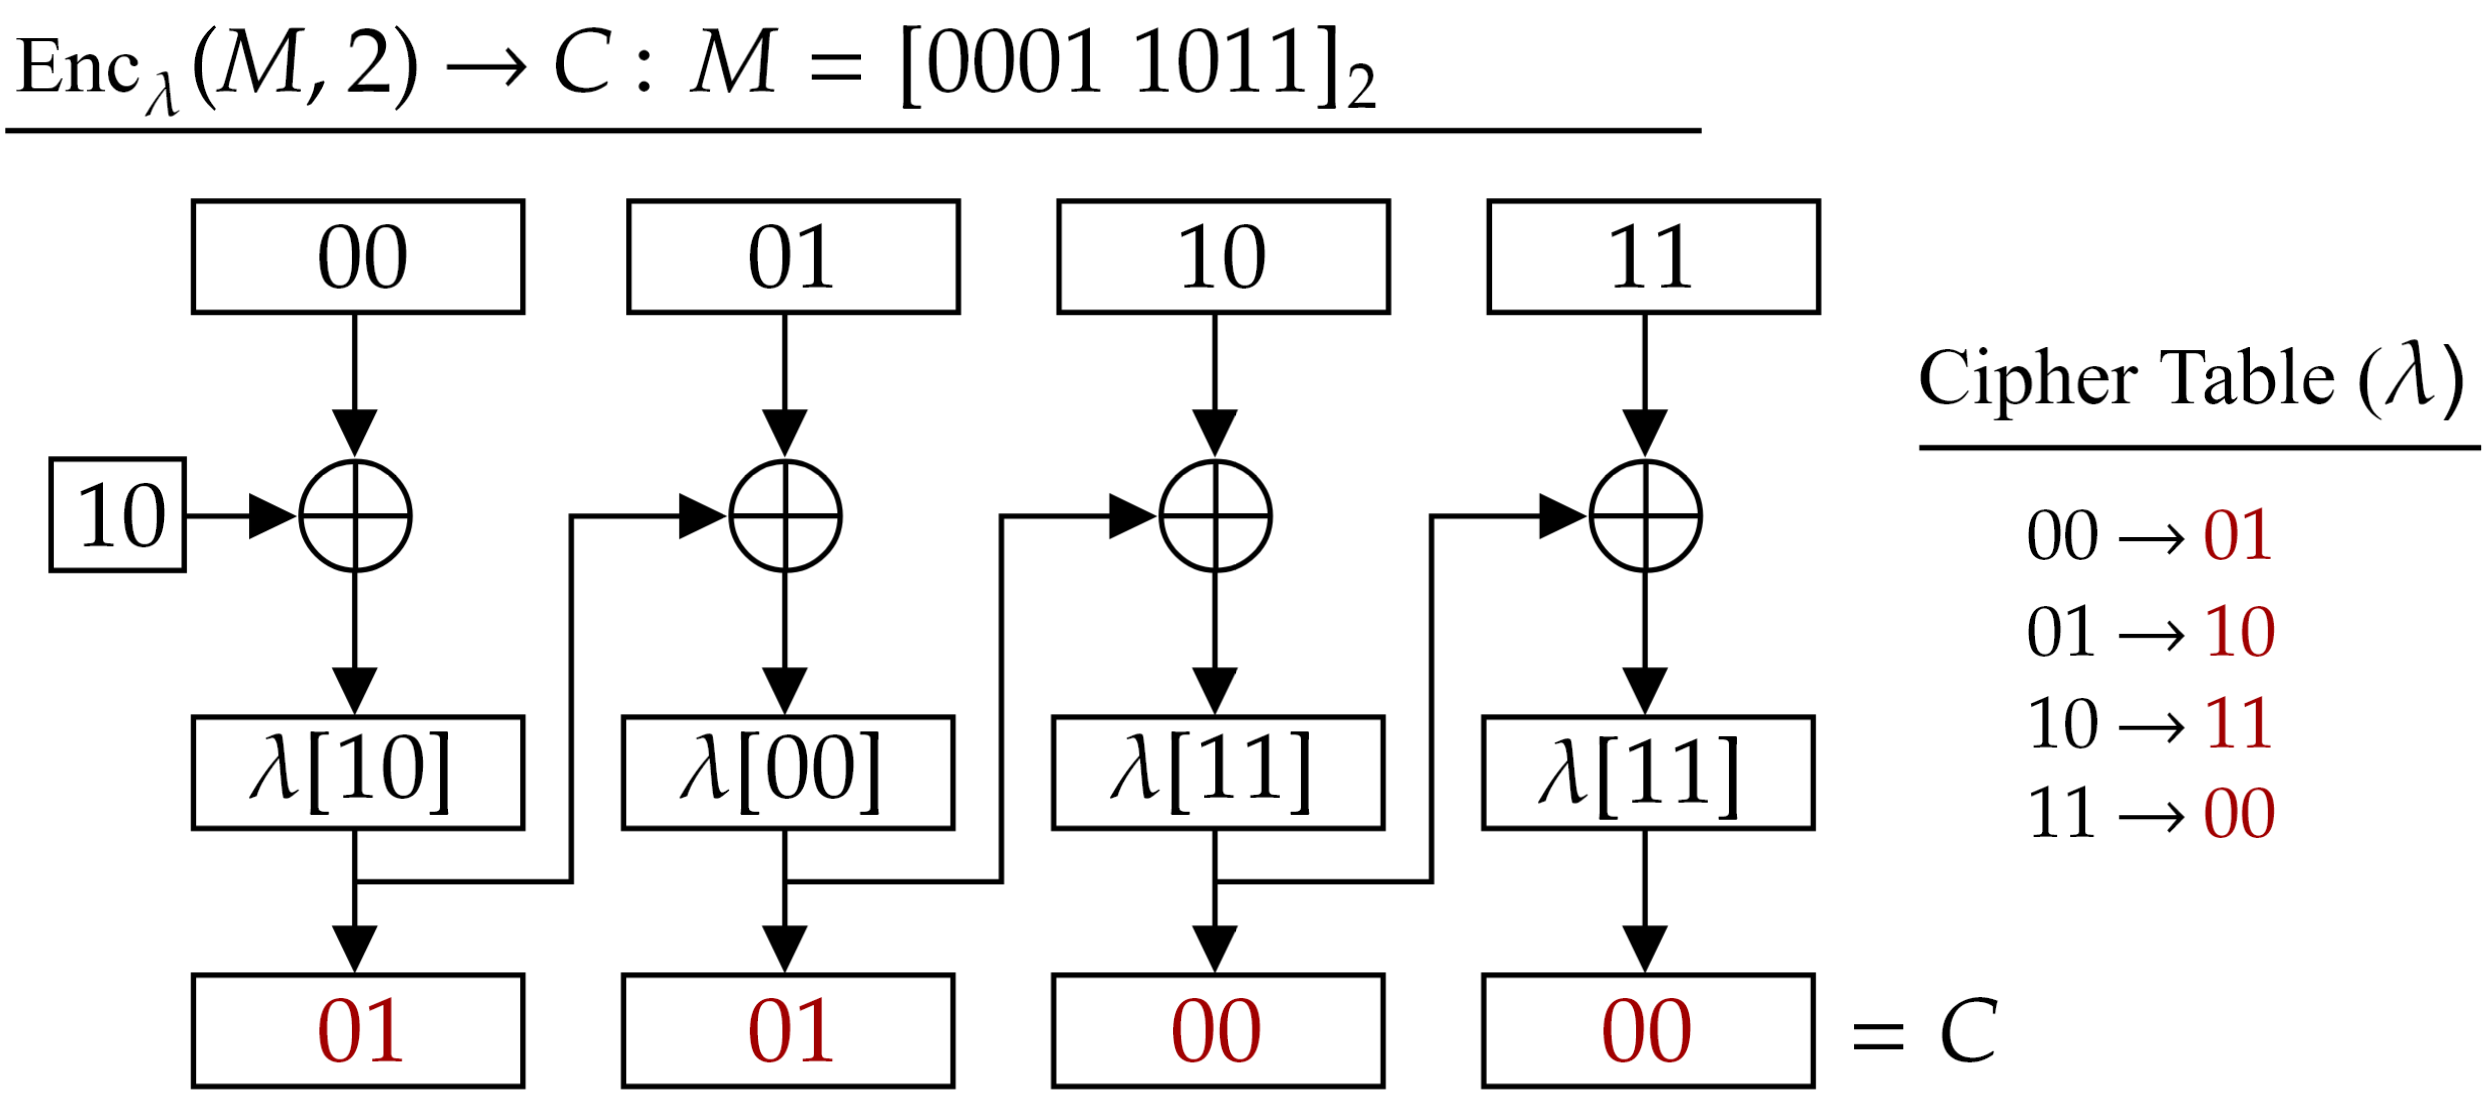
\includegraphics[width=.8\textwidth]{Sections/sec/enc/cbc_ex.png}
    \caption{CBC encryption example with input $[0001\ 1011]_2$ and outputs $[0101\ 0000]_2$.}
    \label{fig:block_cipher}
\end{figure}

\noindent
Plenty of block cyphers elaborate on these concepts. The different flavors are called a \textbf{mode of operation}.

\begin{Def}[Message Authentication Code (MAC)]

    \label{theo:mac}
    A MAC combines a message with a secret key before hashing.
    Let $M$ be the message, $\lambda$ the key, and the function $T\gets$Enc$_\lambda(M)$. Where $T$ is a resulting tag, sometimes called 
    a \textbf{digest} or \textbf{hash}. Then $(M,T)$ is sent over the wire. The receiver also has $\lambda$ and runs Enc$_\lambda(M)$ to verify $T$.\\
    \noindent
    \rule{\textwidth}{0.4pt}
    \textbf{Security Definition}: Integrity and Authenticity. Not confidentiality.
\end{Def}

\newpage 
\noindent
The following figure demonstrates that a MAC protects integrity, as if the message were altered, the receiver would 
not get the same tag with their key. Though an adversary may still intercept and read the message.

\begin{figure}[h!]
    \centering
    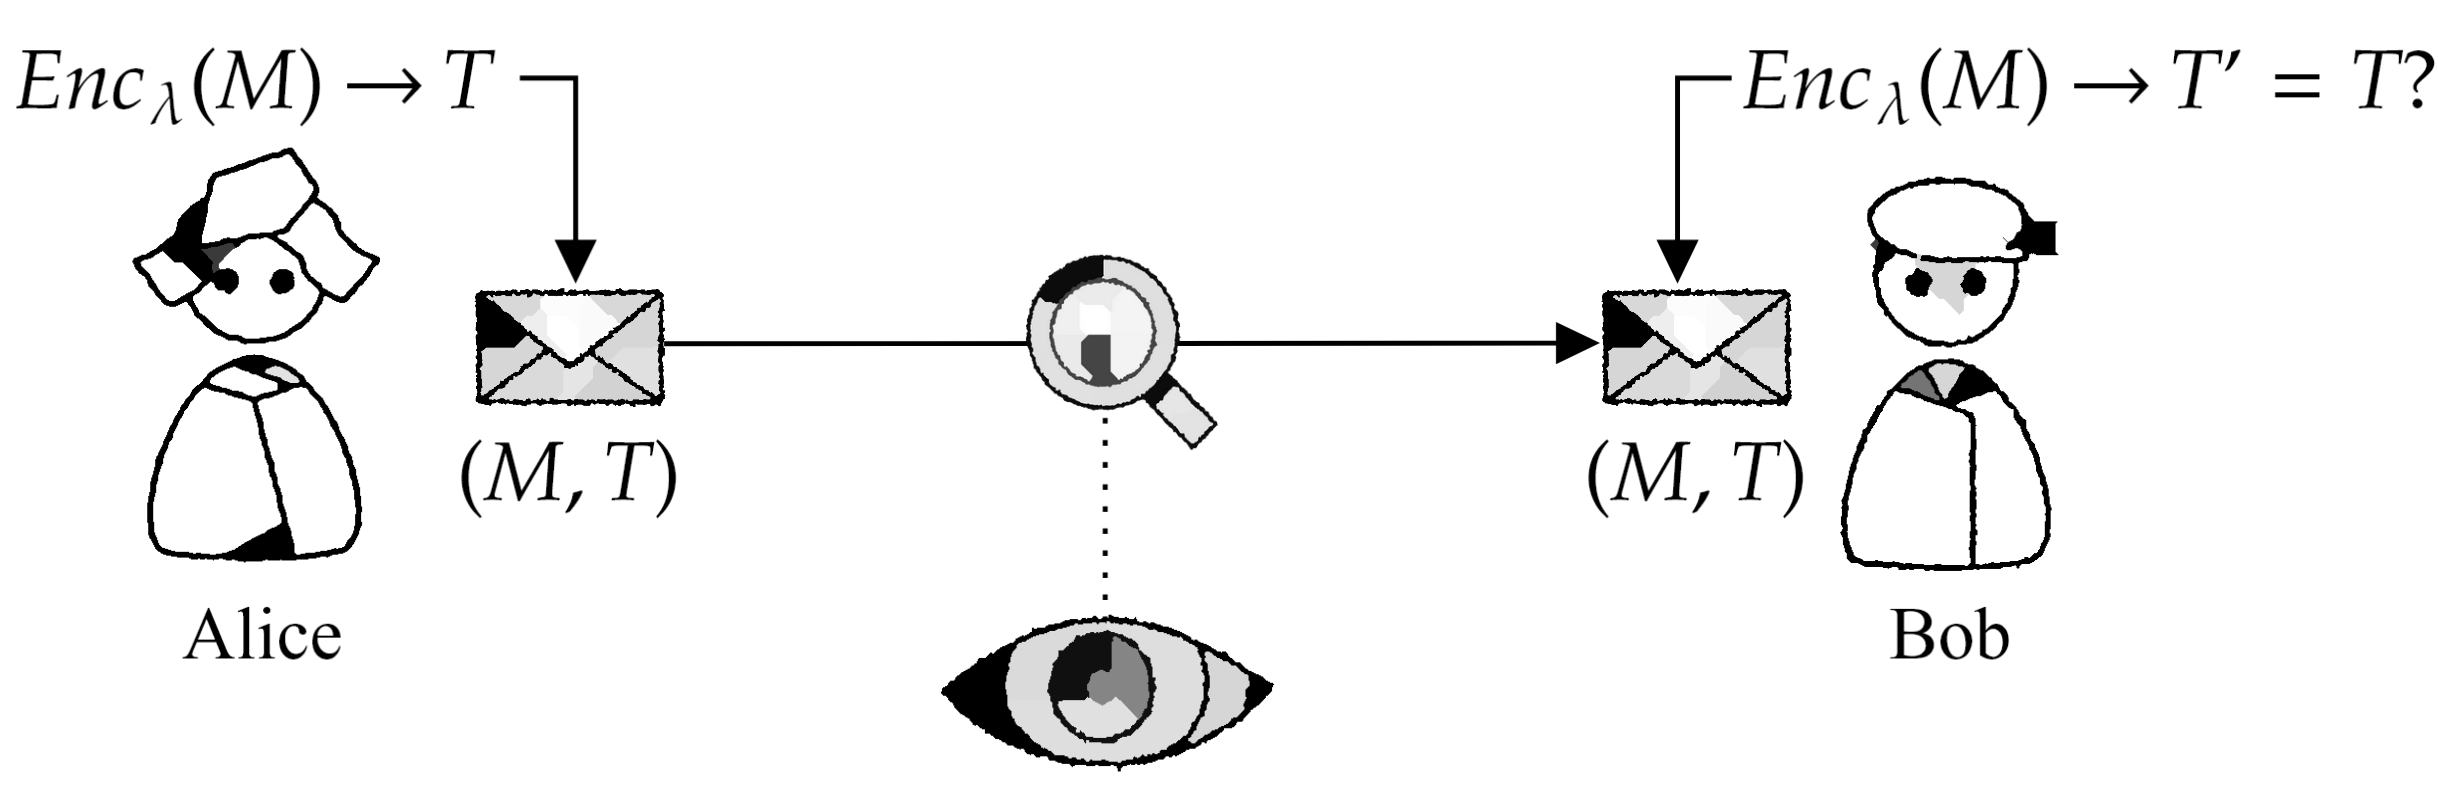
\includegraphics[width=.8\textwidth]{Sections/sec/enc/mac.png}
    \caption{A MAC protecting integrity.}
    \label{fig:block_cipher}
\end{figure}

\begin{theo}[Replay Attack]

    \label{theo:replay_attack}
    A replay attack is when an adversary intercepts a message and resends it to the receiver. The receiver may not know the message was sent twice.
\end{theo}

\begin{figure}[h!]
    \centering
    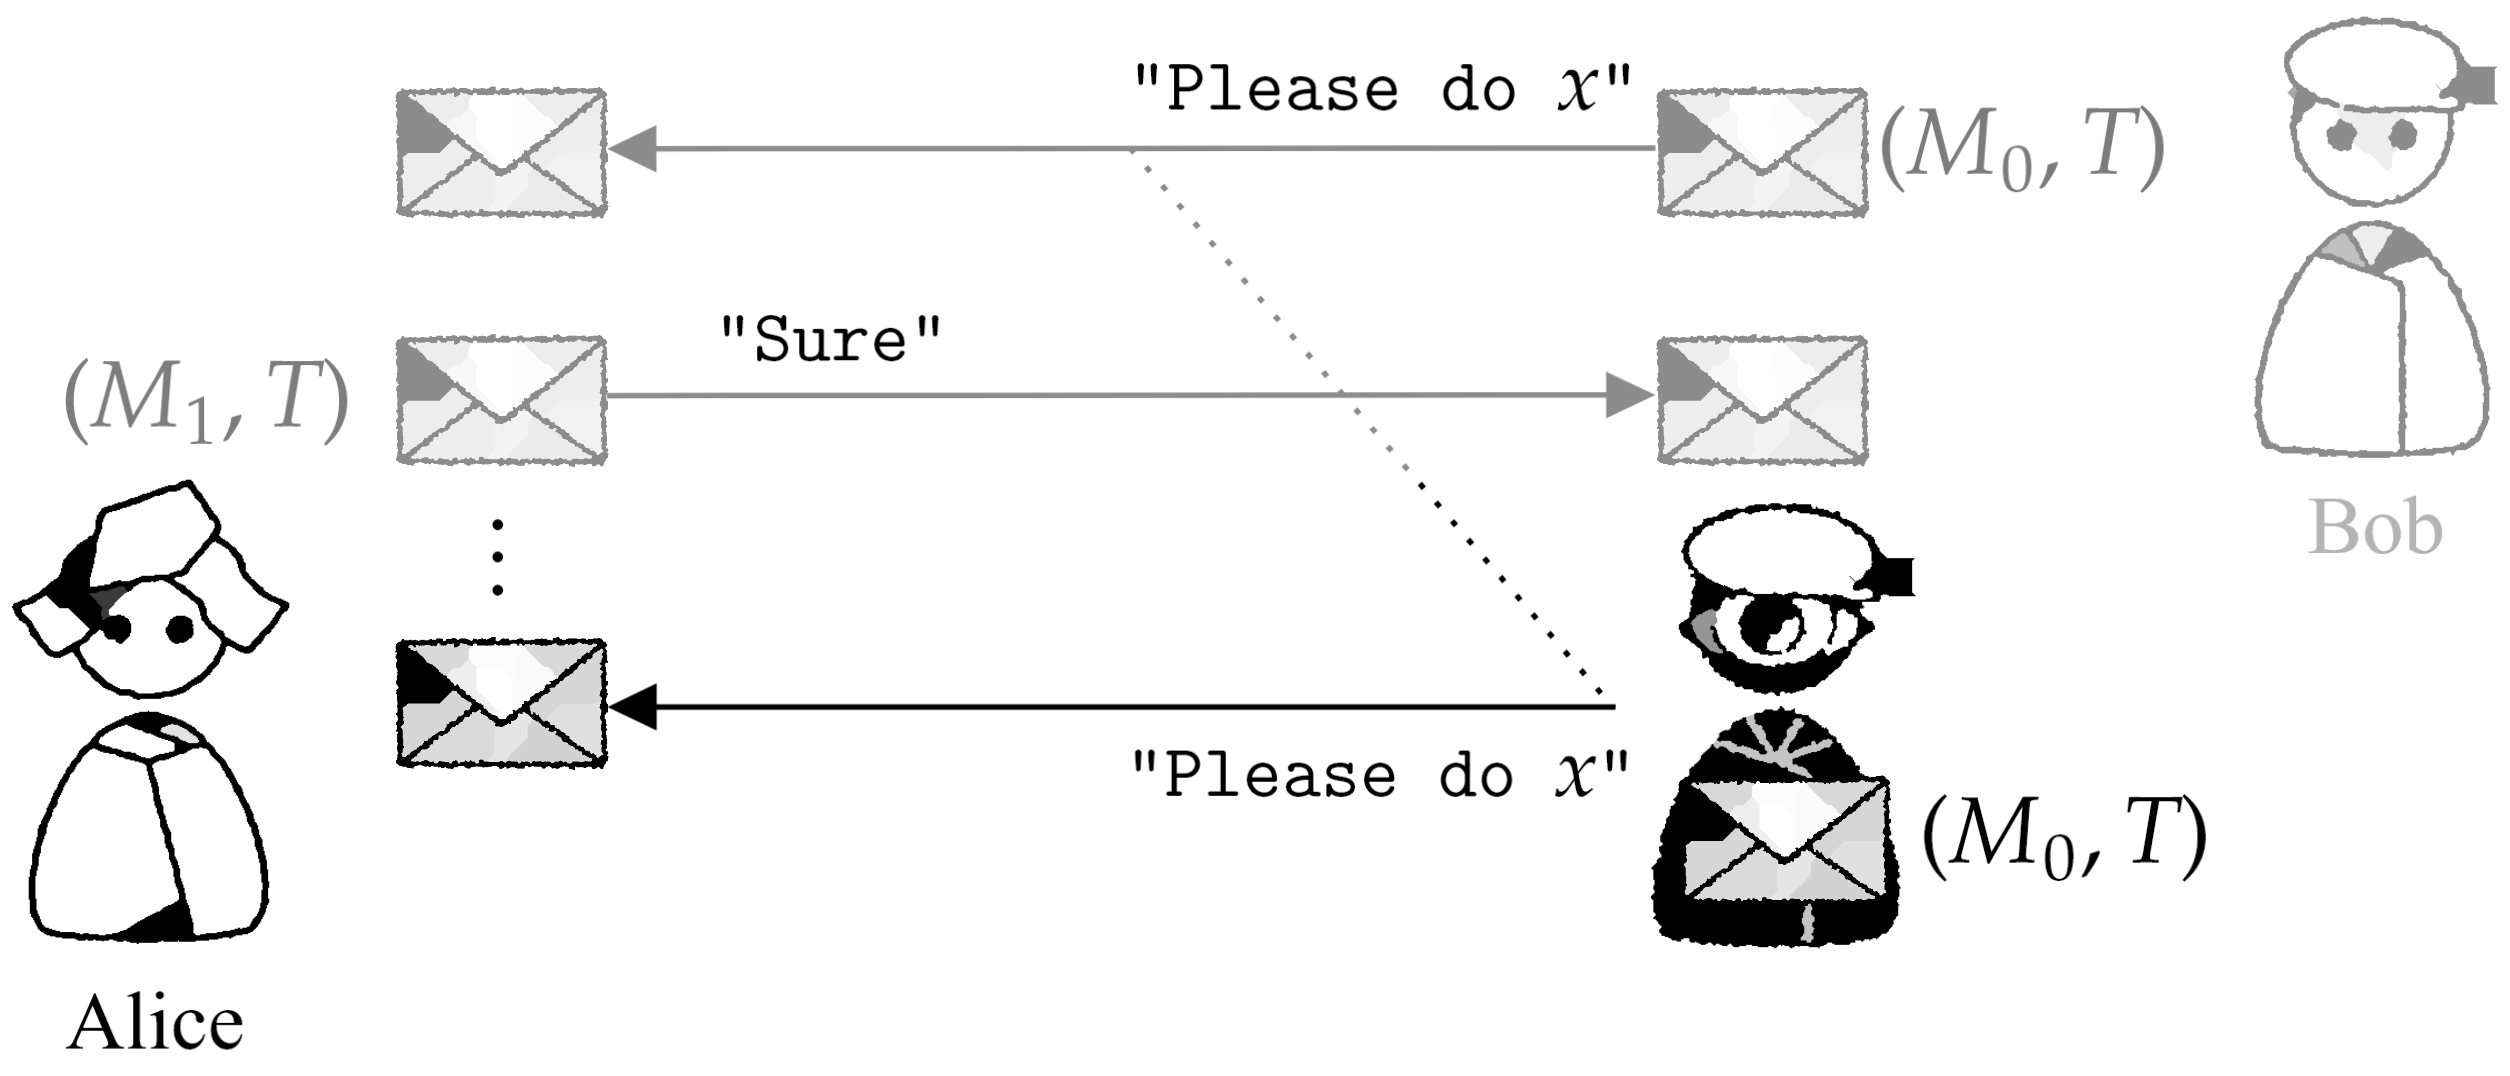
\includegraphics[width=.8\textwidth]{Sections/sec/enc/replay.png}
    \caption{A replay attack, where the adversary intercepts and resends a message.}
    \label{fig:block_cipher}
\end{figure}

\begin{theo}[Replay Attack Prevention]

    \label{theo:replay_attack_prevention}
    To prevent replay attacks, a timestamp or nonce (number used once) is added to the message. The receiver checks the timestamp or nonce to ensure the message is fresh.
\end{theo}

\newpage 

\begin{Def}[Hashed-based Message Authentication Code (HMAC)]

    \label{theo:hmac}
    HMACs are a type of MAC which are standardized and deemed secure. They take a pre-defined 
    hash function (e.g., SHA-256) and apply it to a MAC. I.e., an HMAC is a specific recipe for a MAC. \hfill \cite{seth2013macvsHMAC}
\end{Def}

\section{Block Ciphers \& Modes of Operation}
\begin{Def}[Galios Counter Mode (GCM)]

    \label{theo:gcm}
    GCM uses a MAC called GMAC, which is a variant of the HMAC. It encrypts data 
    with a desired Encryption Algorithm and then GMACs (MACs) the data into cipher text. The final hash is the tag. This 
    process goes as follows:
    \begin{itemize}
        \item \textbf{Encryption}:
        \begin{enumerate}
            \item Each block of plaintext is XORed with the encryption key.
            \item To ensure randomness, a counter is added to each encryption before XORing.
            \item To ensure randomness of the counter, an IV is added to it.
        \end{enumerate}
        \item \textbf{MAC}:
        \begin{enumerate}
            \item After encryption, the data is XORed with a previous hash then GMACed.
            \item The GMAC is then used to XOR the next block's cipher before hashing again.
            \item To start the chain of XORing, a 128-bits of zeros is encrypted and GMACed.
            \item After the final block, the length of the message is XORed with the prior hash, then GMACed.
            \item Finally, an encryption of 32-bits of zeros is XORed with the final hash, producing the tag.
        \end{enumerate}
    \end{itemize}

    \noindent
    GCM also supports \textbf{Authentication of Additional Data (AAD)}, which is data that is not encrypted but is still hashed.
    So in addition to authenticating and encrypting a message, GCM can also authenticate additional unencrypted data.
    If GCM is only used for authentication, it is called \textbf{GMAC}. \hfill \cite{vidder_gcm_gmac}
    \noindent
    \rule{\textwidth}{0.4pt}
    \textbf{Security Definition}: Confidentiality, Integrity, and Authenticity.
\end{Def}

\vfill
\begin{center}
    \textit{GCM Diagram and Elaborations on the next page.}
\end{center}
\vfill 

\newpage

\noindent
The following figures are first broken up and then combined for clarity.\\

\begin{figure}[h!]
    \centering
    \hfill{1em}
    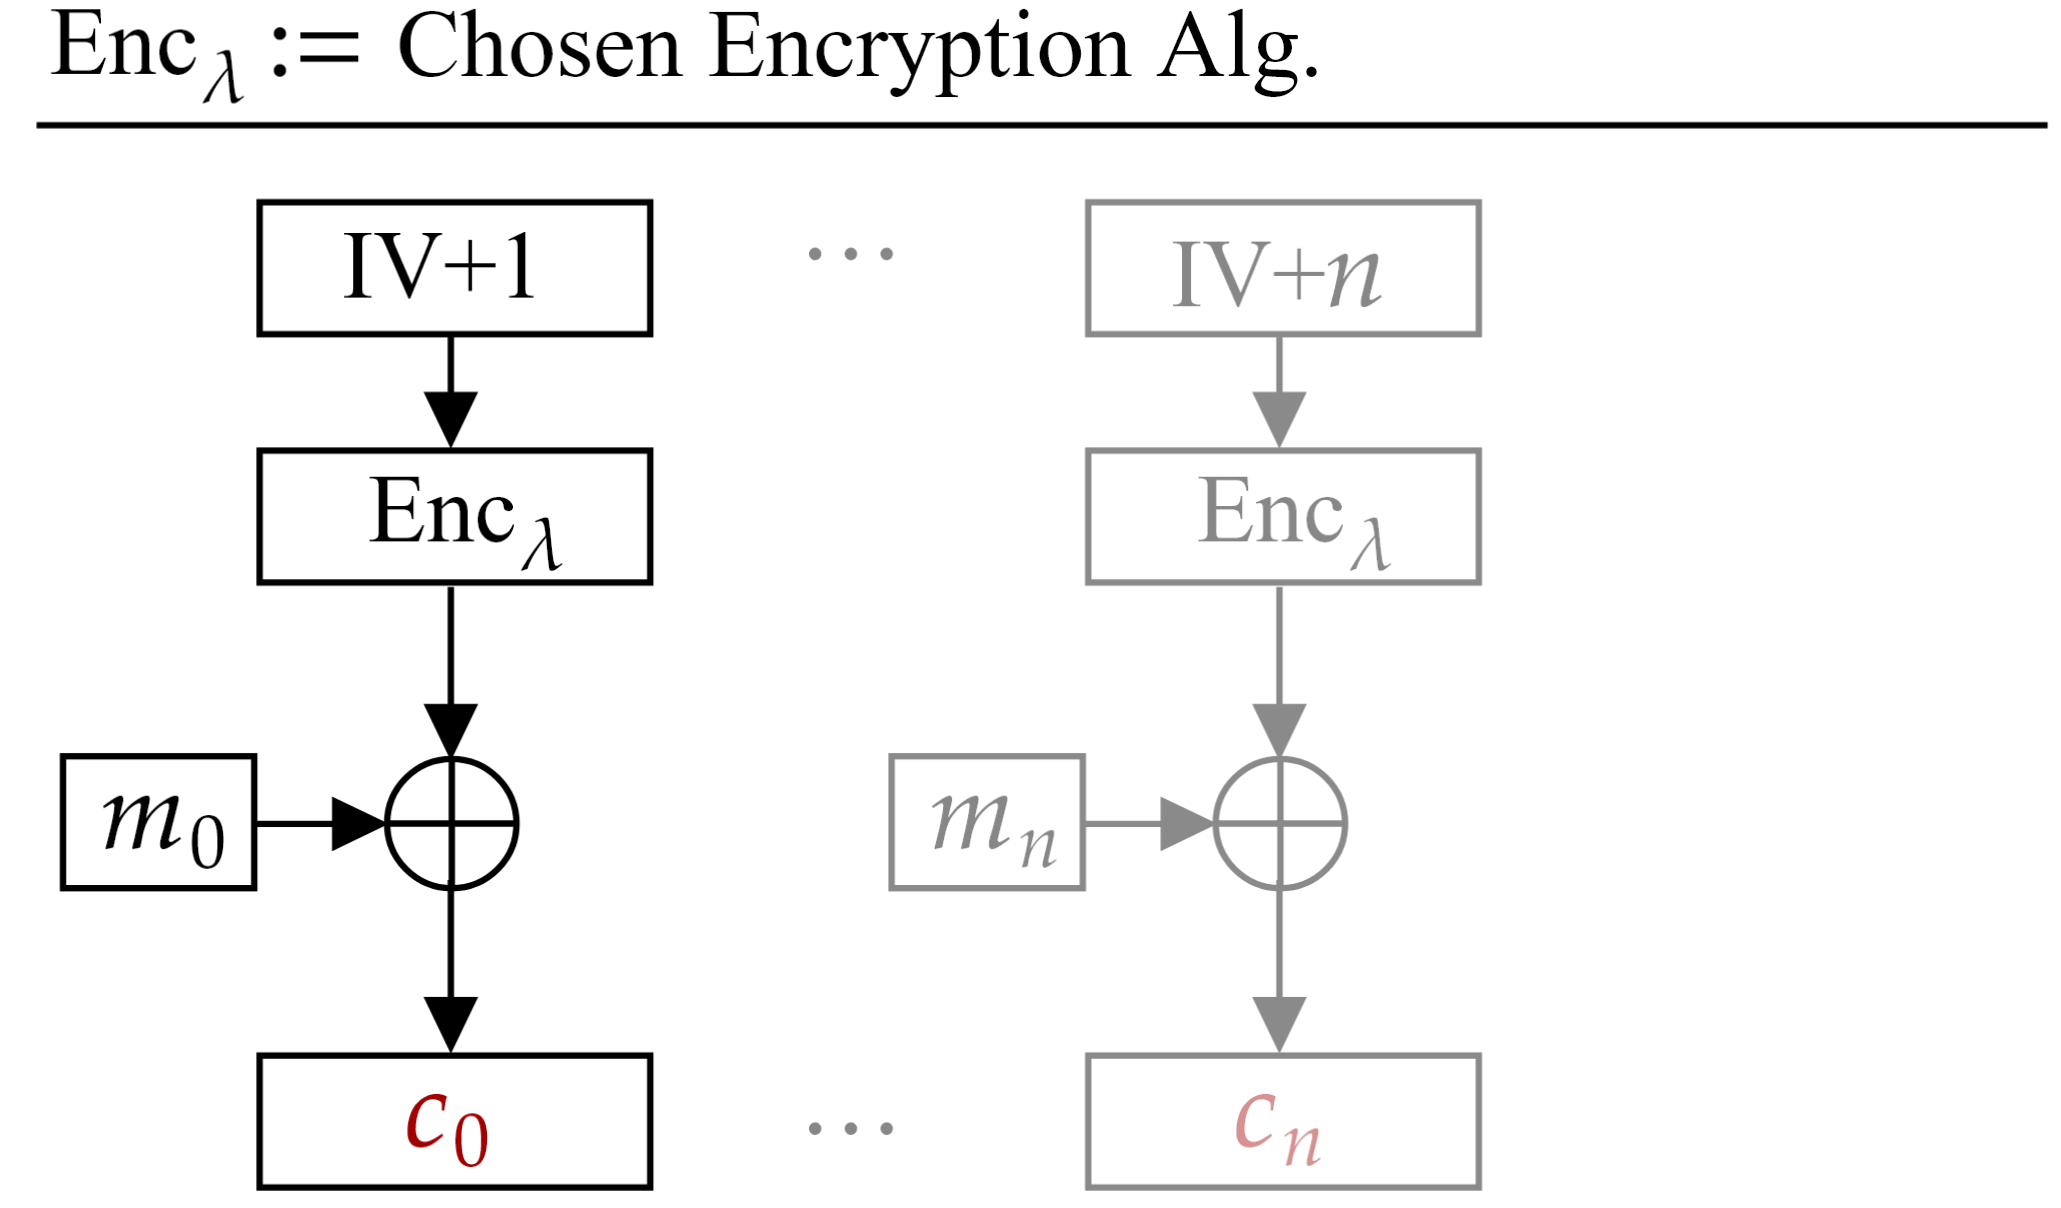
\includegraphics[width=.8\textwidth]{Sections/sec/enc/iv.png}
    \caption{GCM IV and Counter XORing with Plaintext to create Ciphertext.}
    \label{fig:block_cipher}
\end{figure}

\begin{figure}[h!]
    \centering
    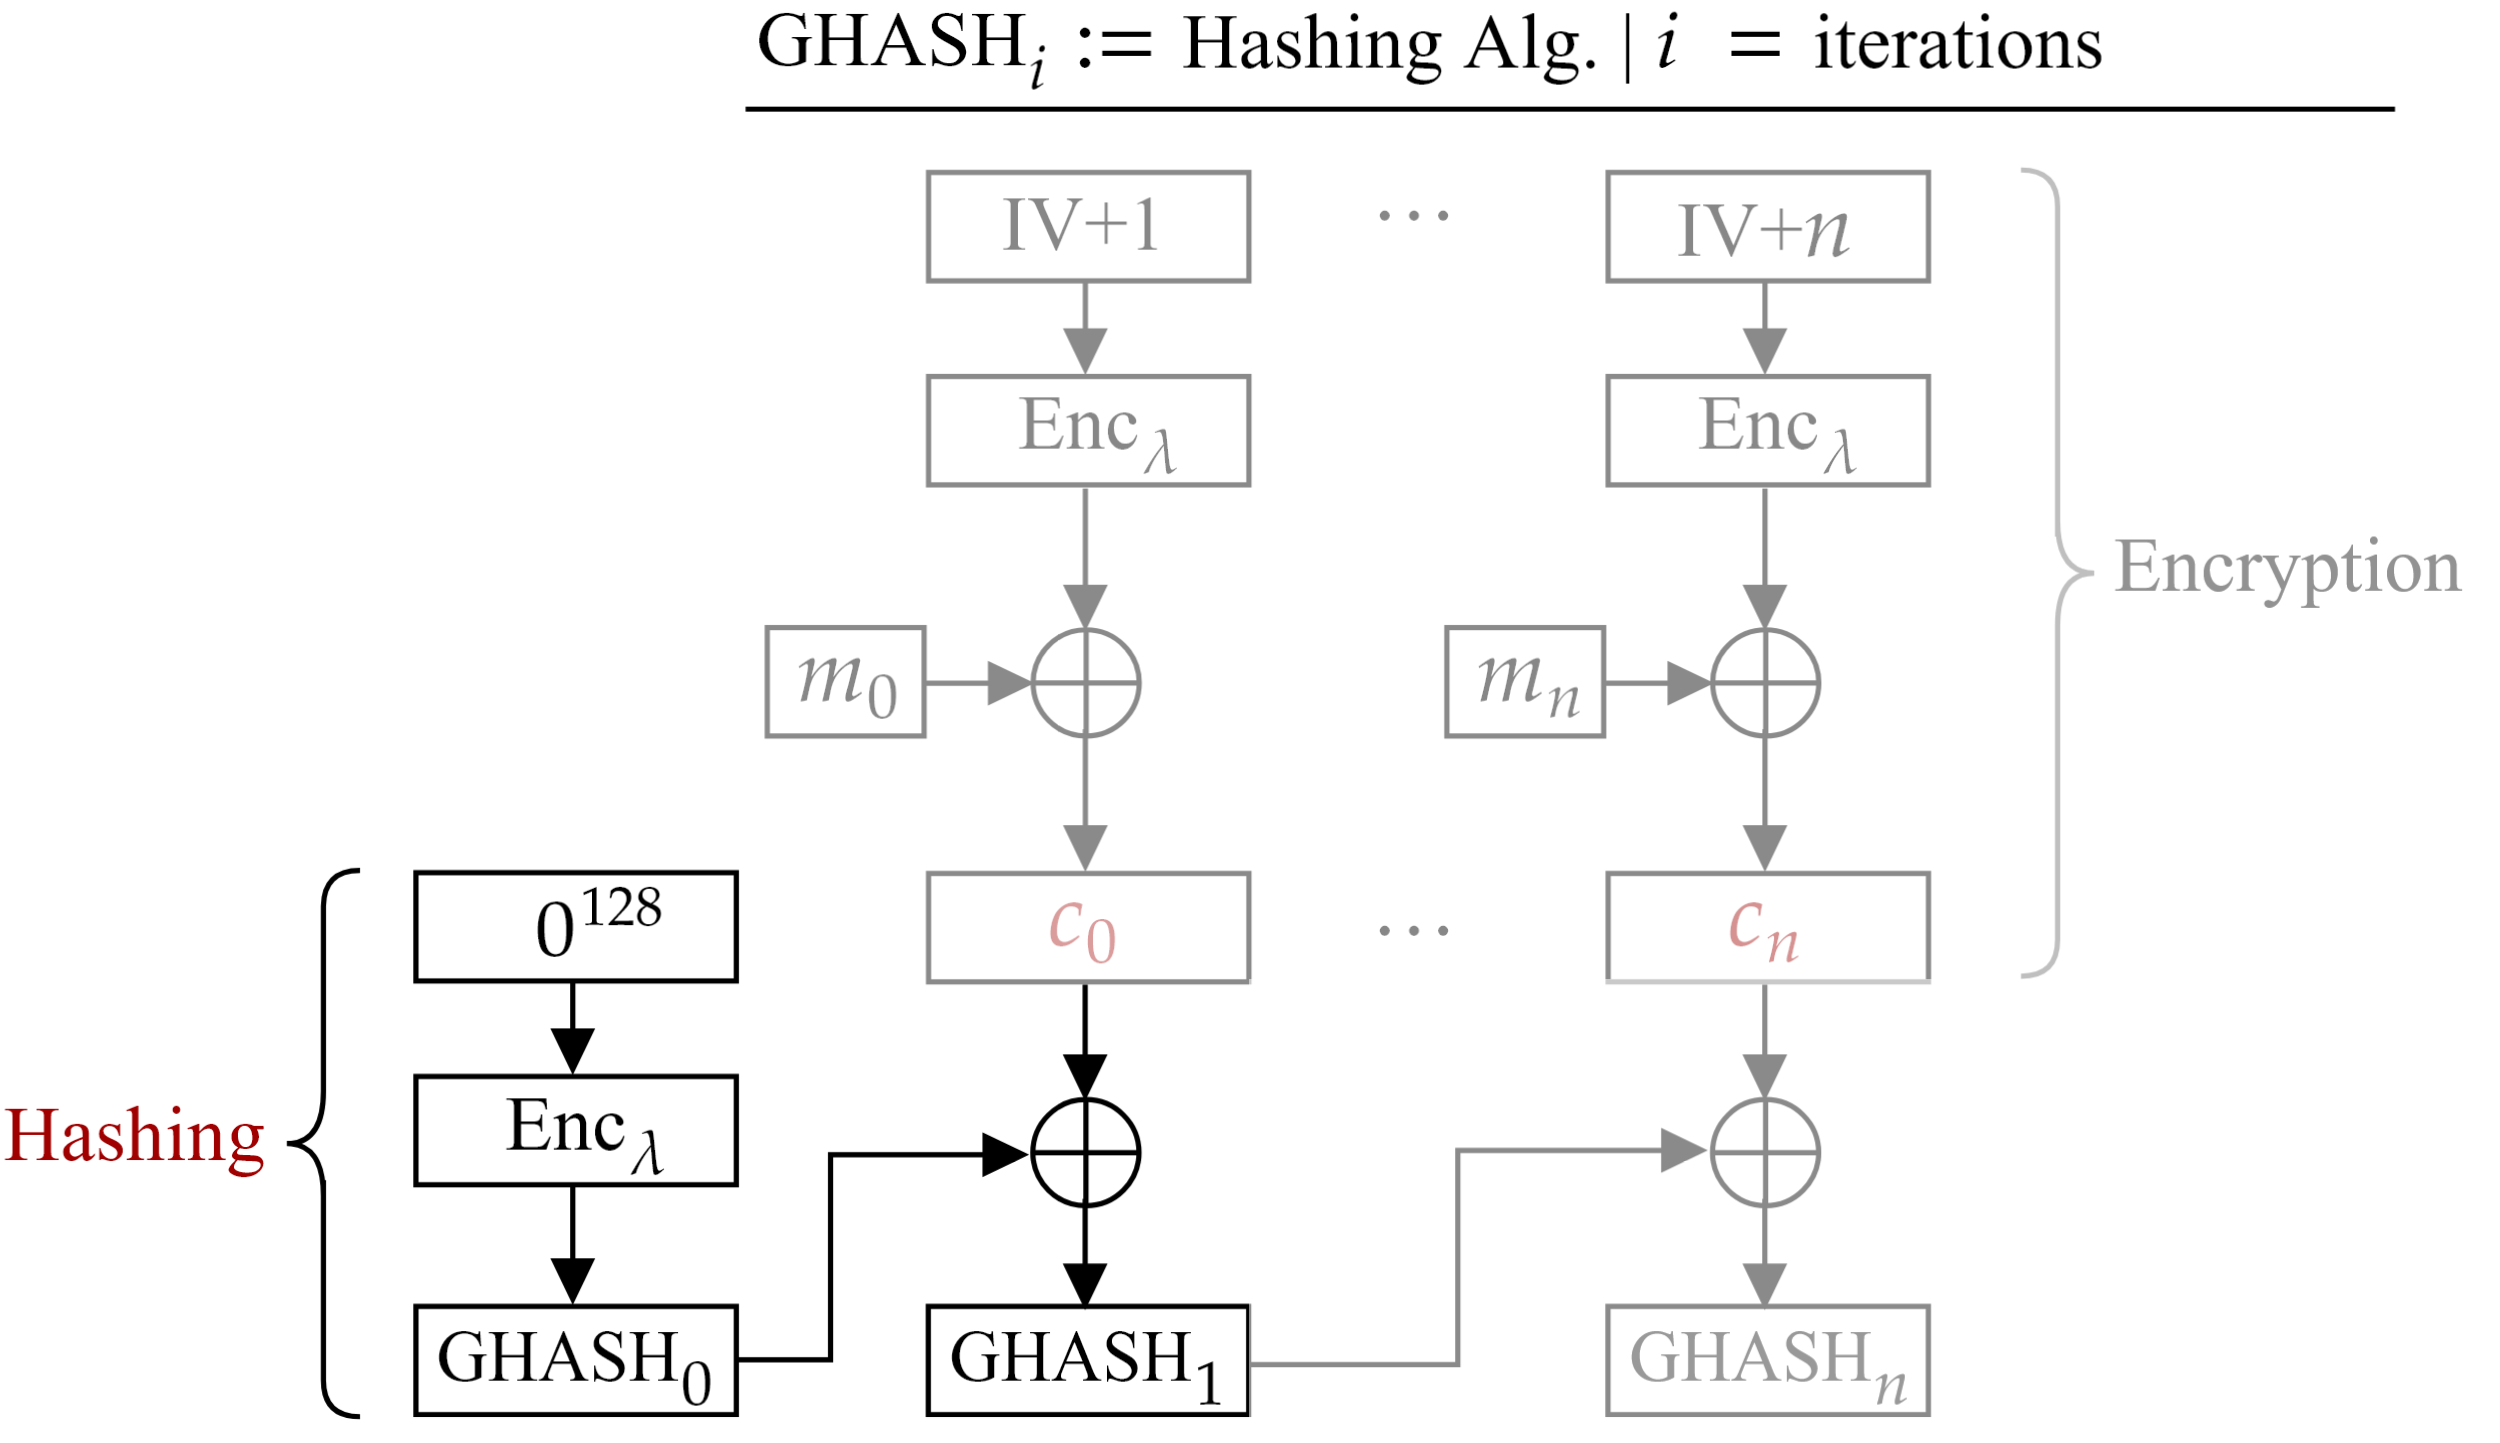
\includegraphics[width=.9\textwidth]{Sections/sec/enc/ghash.png}
    \caption{128-bits of zeros is encrypted and GMACed, starting the chain of XOR hashing.}
    \label{fig:block_cipher}
\end{figure}
\vfill
\begin{center}
    \textit{Continued on the next page.}
\end{center}
\vfill 
\newpage 

\noindent
To finish the chain of XOR hashing:
\begin{figure}[h!]
    \centering
    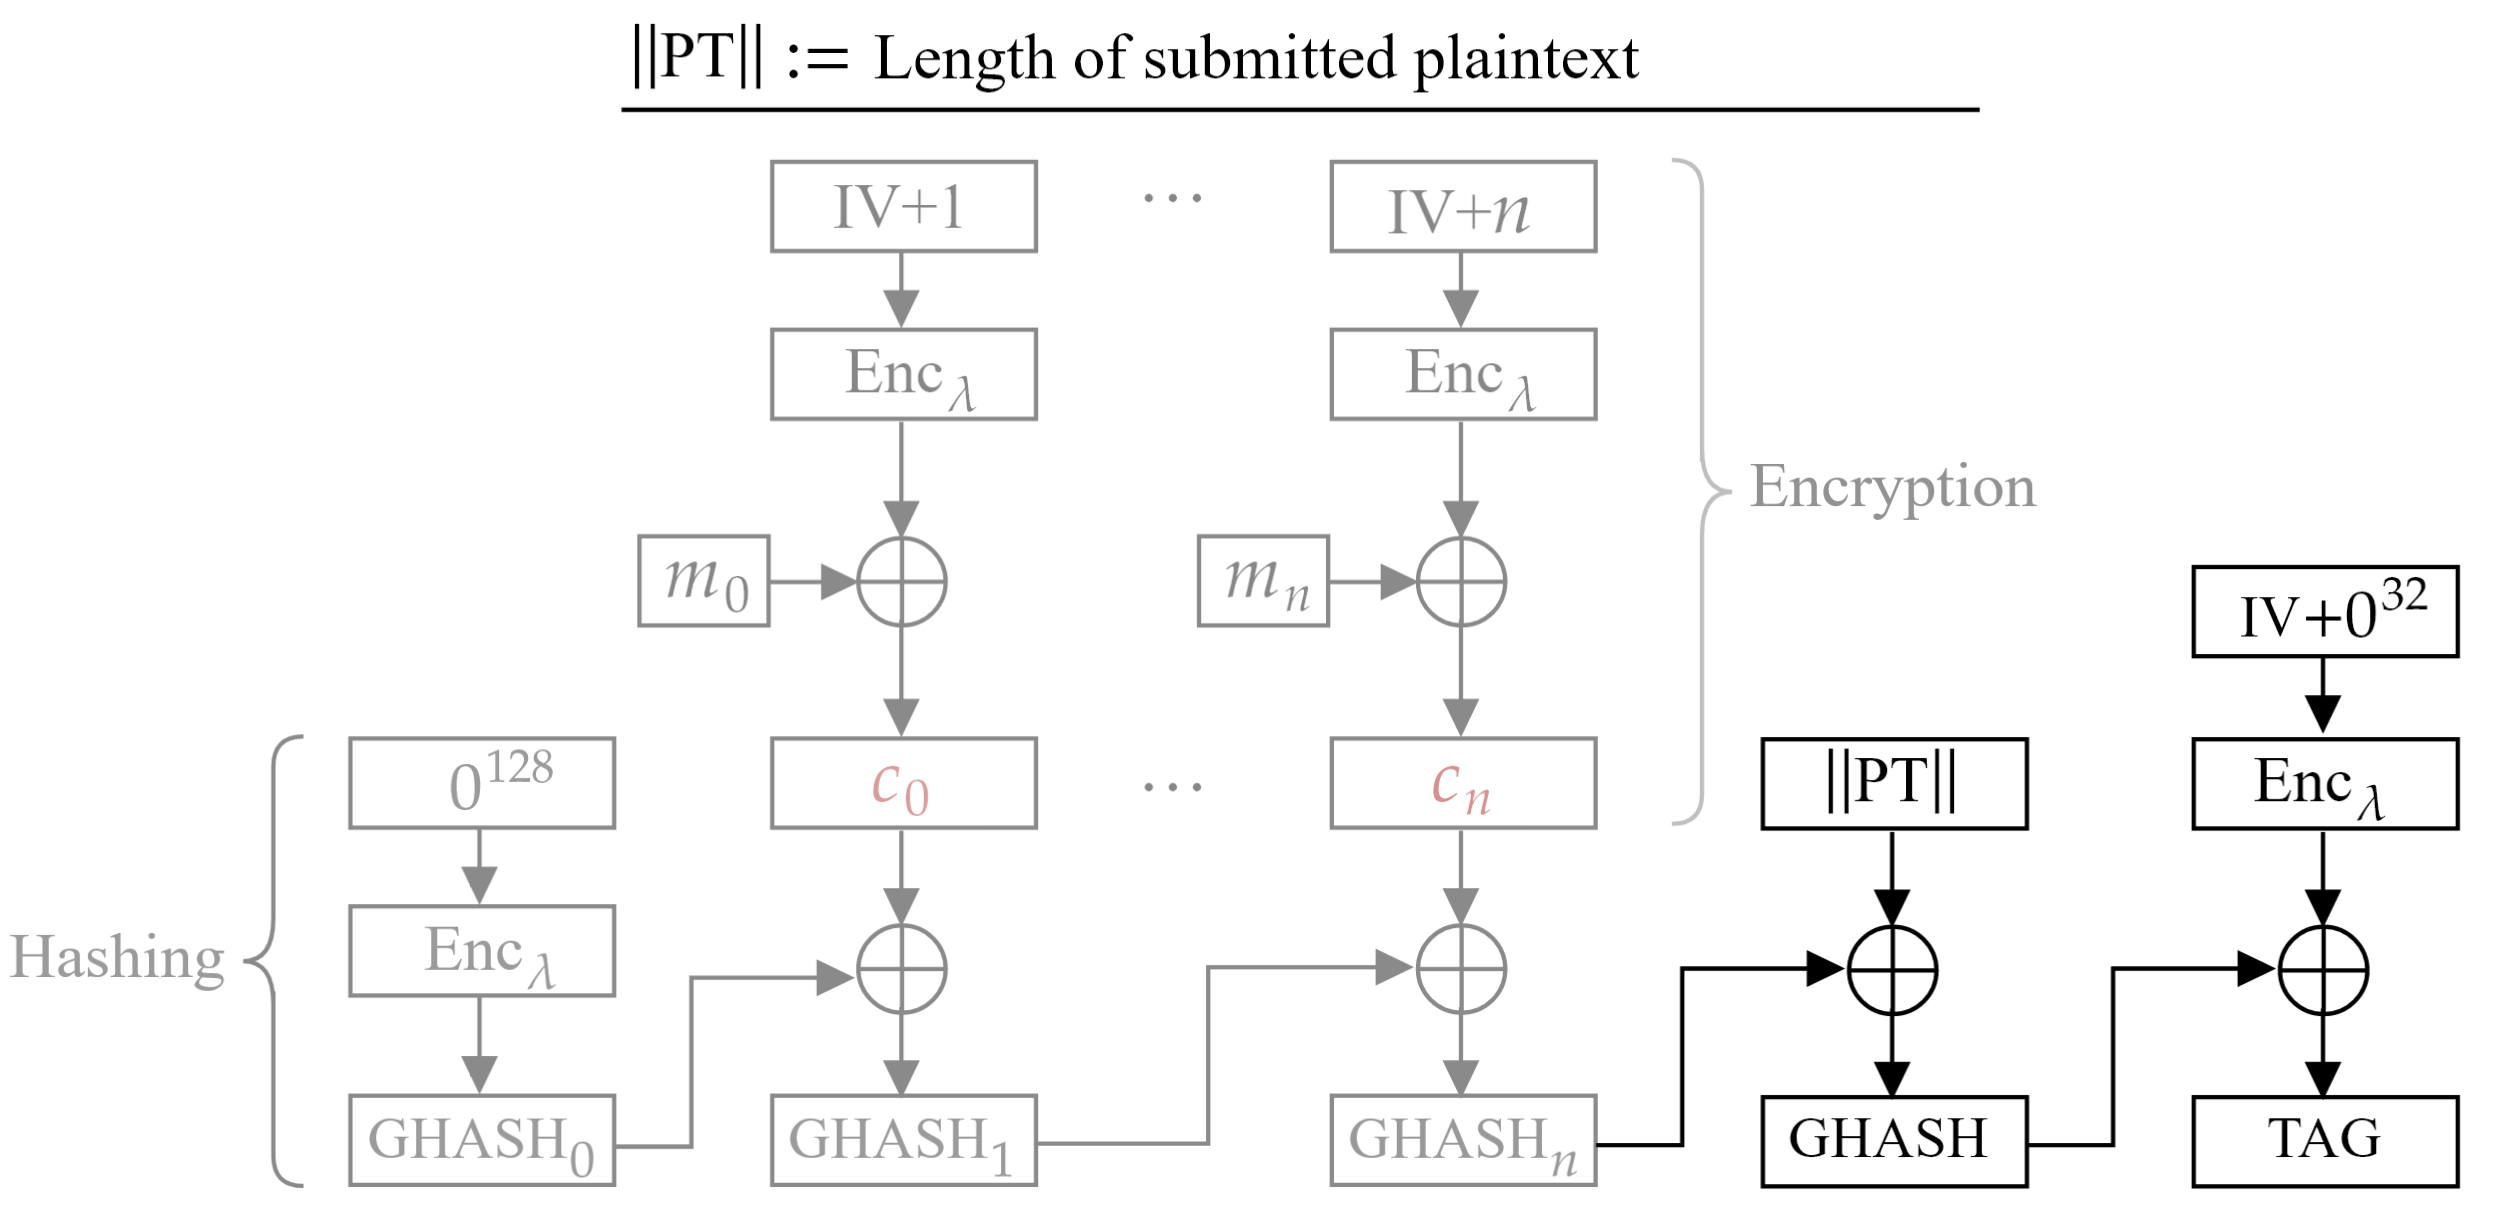
\includegraphics[width=1\textwidth]{Sections/sec/enc/len.png}
    \caption{The length of the message is XORed with the prior hash, then GMACed with 32-bits of encrypted zeros concatenated with the IV.}
    \label{fig:block_cipher}
\end{figure}

\begin{figure}[h!]
    \centering

    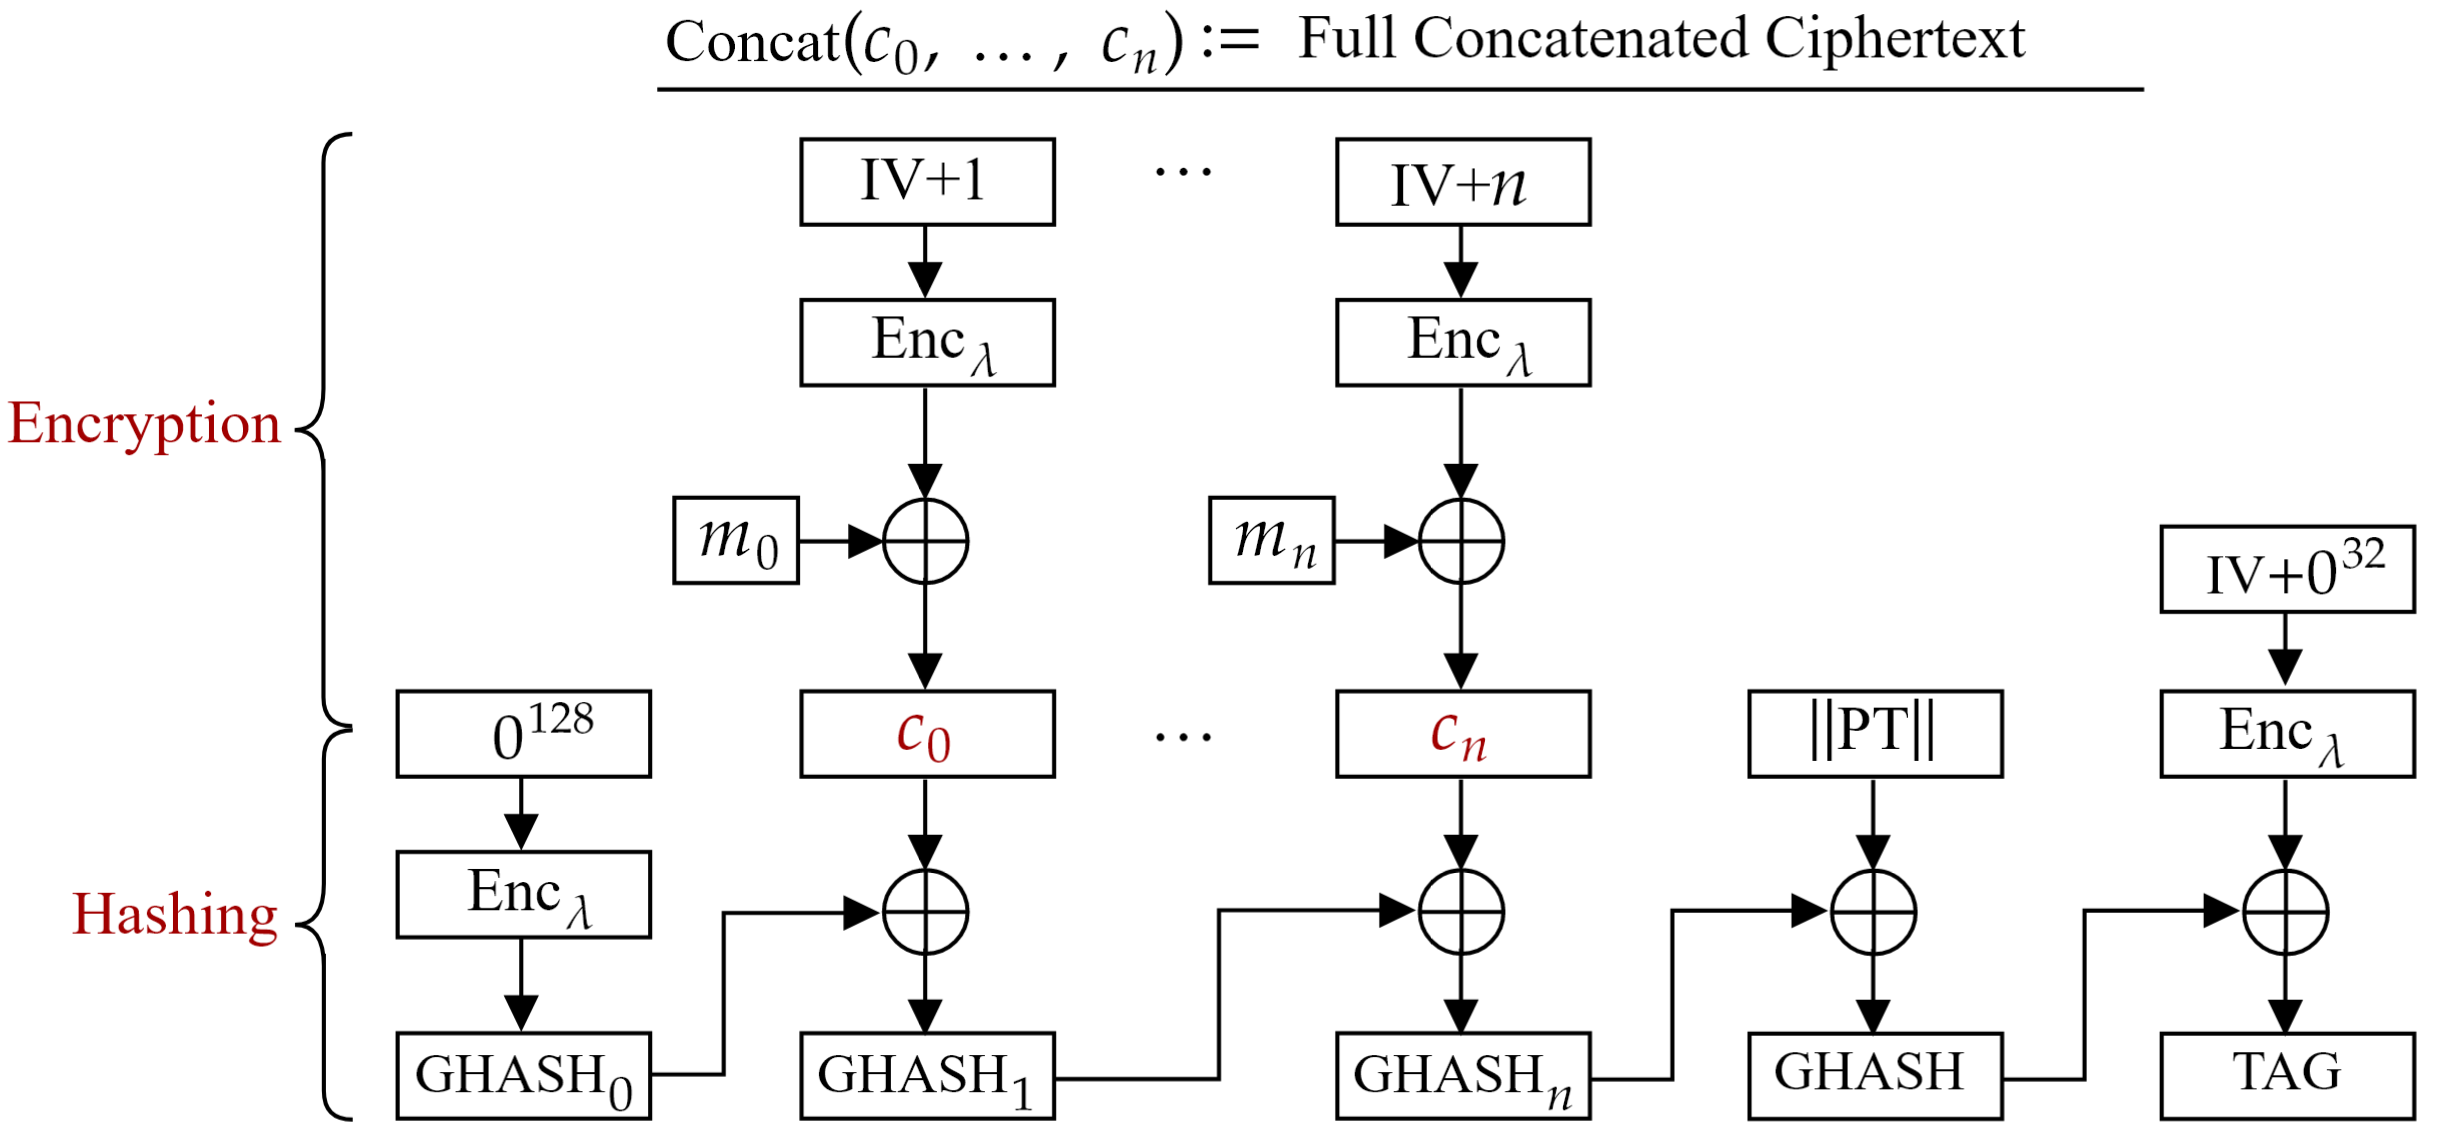
\includegraphics[width=1\textwidth]{Sections/sec/enc/semi.png}
    \caption{A semi complete GCM diagram (Encryption and Authentication), with AAD left out.}
    \label{fig:block_cipher}
\end{figure}
\noindent
\vfill
\begin{center}
    \textit{Continued on the next page.}
\end{center}
\vfill 
\newpage

\noindent
A full GCM diagram with AAD:
\begin{figure}[h!]
    \centering
    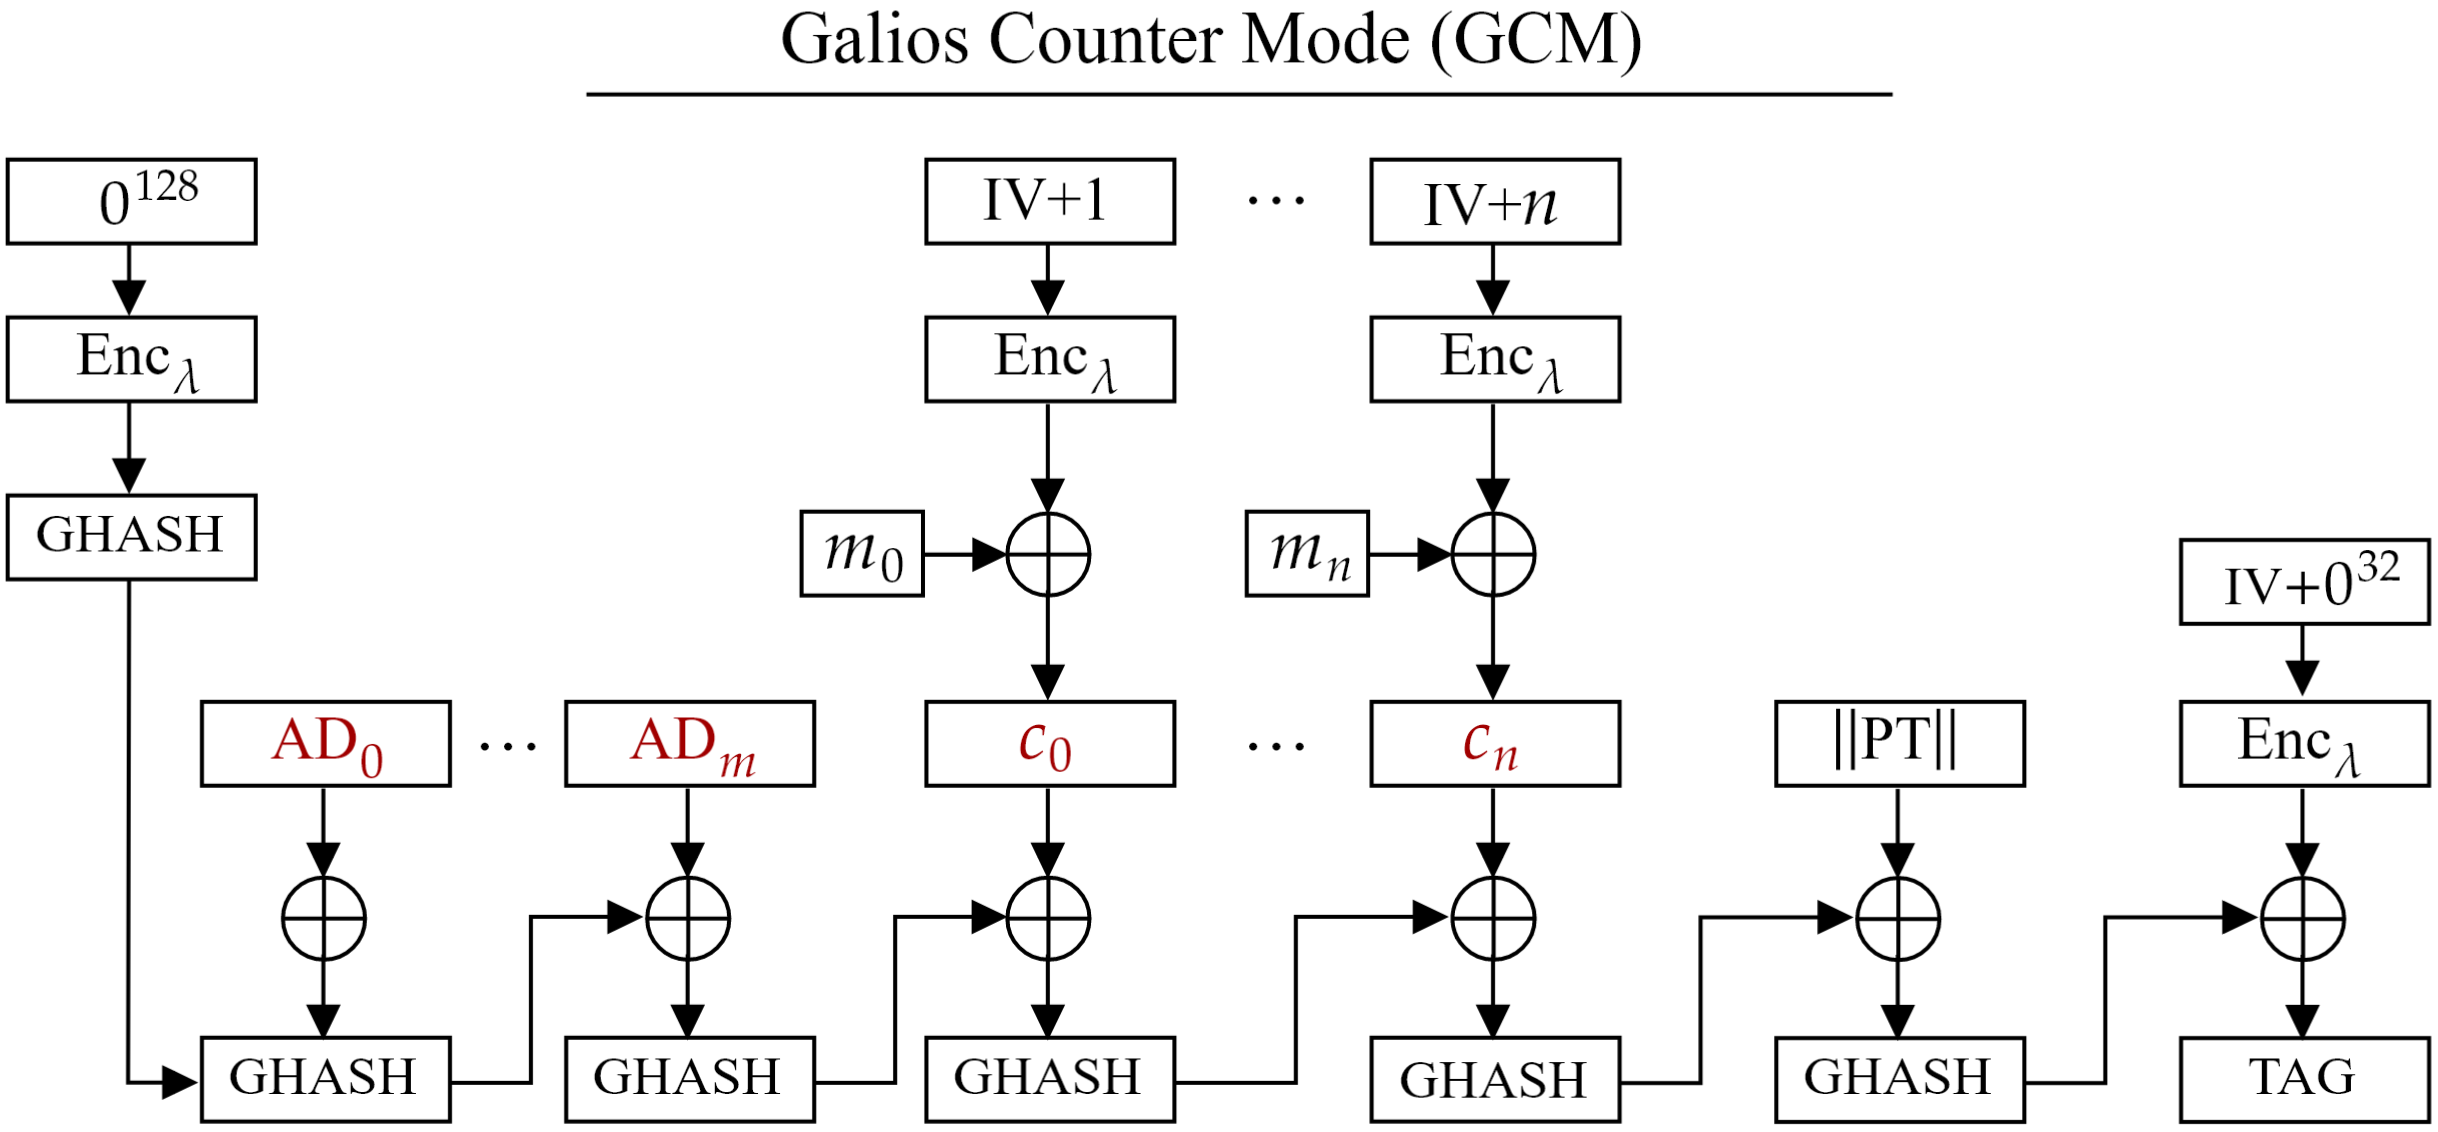
\includegraphics[width=1\textwidth]{Sections/sec/enc/gcm.png}
    \caption{A full GCM diagram: Encryption, Authentication, and unencrypted Additional Authenticated Data (AAD).}
    \label{fig:block_cipher}
\end{figure}

